\chapter{\label{cha:par-str}Partition Strategies}
\section{Motivation}
To optimize the performance of Dan Suciu's algorithm, multiple tests were done as described in preceding chapters. The graph was partitioned by default rules, which means that if there are four partitions and 100 nodes, we put node 1-25 into the first partition, 26-50 into the second partition, etc. An interesting finding is that for most queries, the Step 2 in the modified Dan Suciu's Algorithm only runs for one iteration, which indicates all paths in Global Accessible Graph (GAG) collected are of length 1. This reflects that every site only filters all edges that can be part of the result and returns them immediately without doing any local search. The reason behind this is that with a bad partitioner, the search process can easily reach the output node and stop searching. By using a smart partitioner, the distributed search processes run much more iterations, and the size of the GAG is reduced significantly. Thus in this chapter, we firstly observe the relationship between number of input-nodes or cross-edges and the GAG size, then give the theoretical size of GAG in the form of input-nodes number. In the evaluation section, we verify the formulas by running modified Dan Suciu's algorithm against GMark Benchmark graphs which are partitioned by different partitioners.
\section{Observations}
In figure \ref{fig:alibaba-Random-Queries}, we show the testing result for eight random queries from Alibaba benchmark. The application is run with three partitioners: random partitioner, default (ordered) partitioner and METIS partitioner. We choose the GAG size as primary observation target since it's the only data transmitted in theory, affecting network communication as well as computation time.  
\begin{figure}[h!]
  \caption{GAG Size of Random Queries}
  \label{fig:alibaba-Random-Queries}
  \centering
    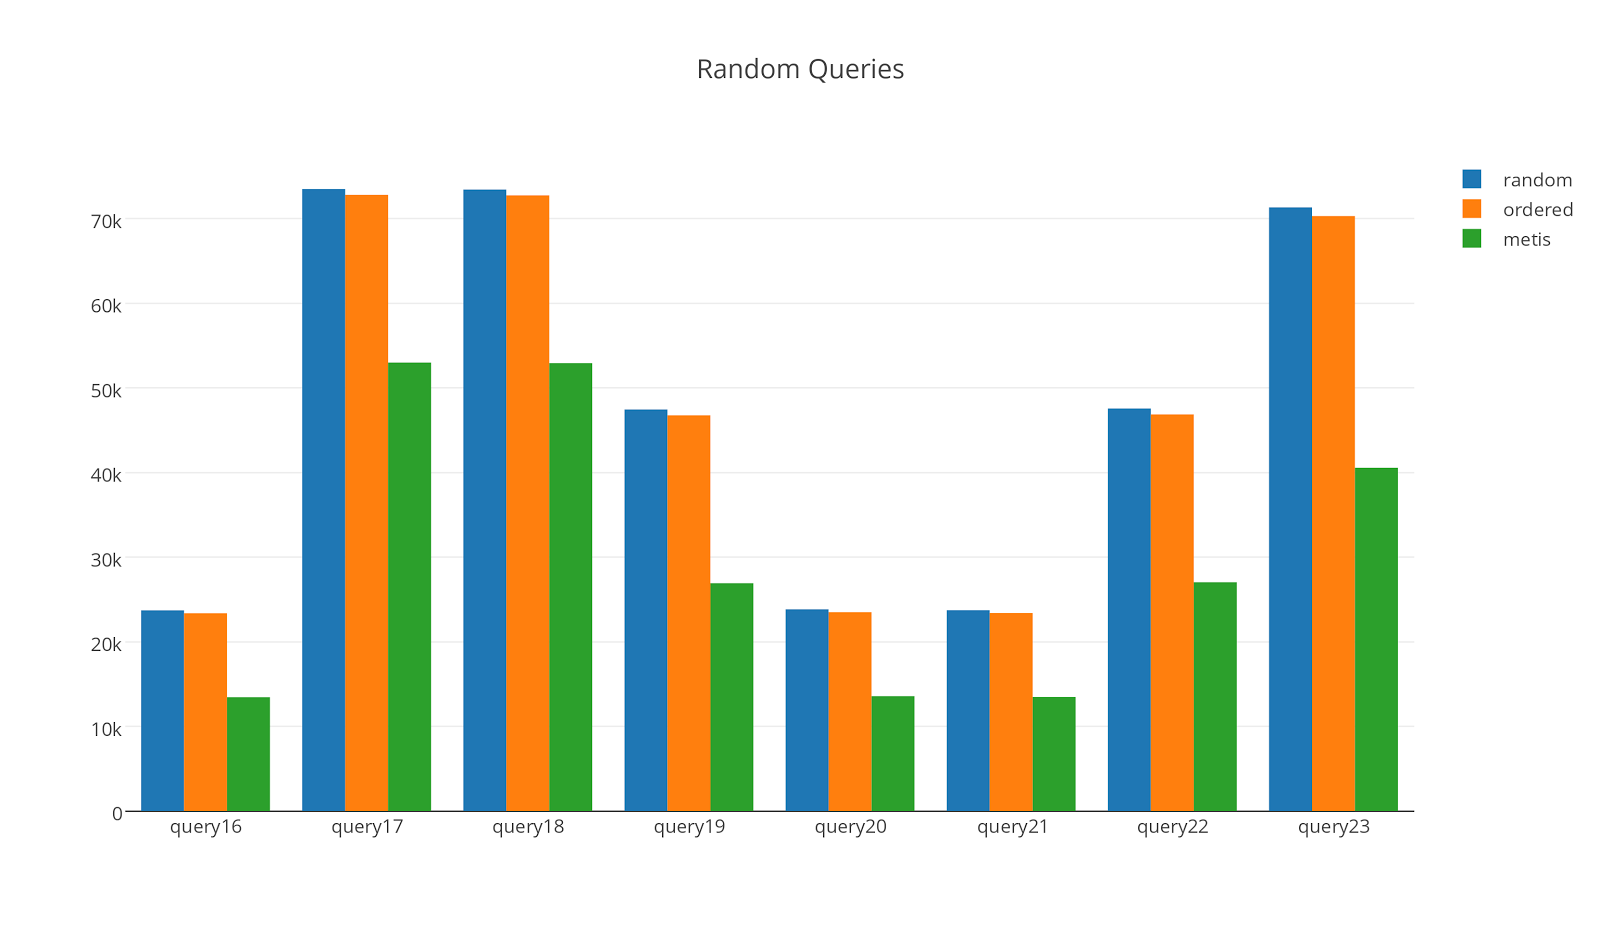
\includegraphics[width=0.8\textwidth]{img/alibaba-Random-Queries}
\end{figure}
\\It turns out that the METIS partitioner can reduce the size of GAG by $30\%-50\%$ comparing to other two partitioners. As mentioned in research background, the METIS algorithm intends to minimize the number of cross-edges while here it turns out that the size of the GAG is not correlated to cross-edges, but the number of input-nodes: In Figure \ref{fig:alibaba-structure}, we can see METIS is not better than the default partitioner in the number of cross-edges, but halves the number of input-nodes. Moreover, the ordered partitioner has much fewer cross-edges than the random partitioner, but still produces a similar size of GAG.
\begin{figure}[h!]
  \caption{Basic Stats for Different Parititioners}
  \label{fig:alibaba-structure}
  \centering
    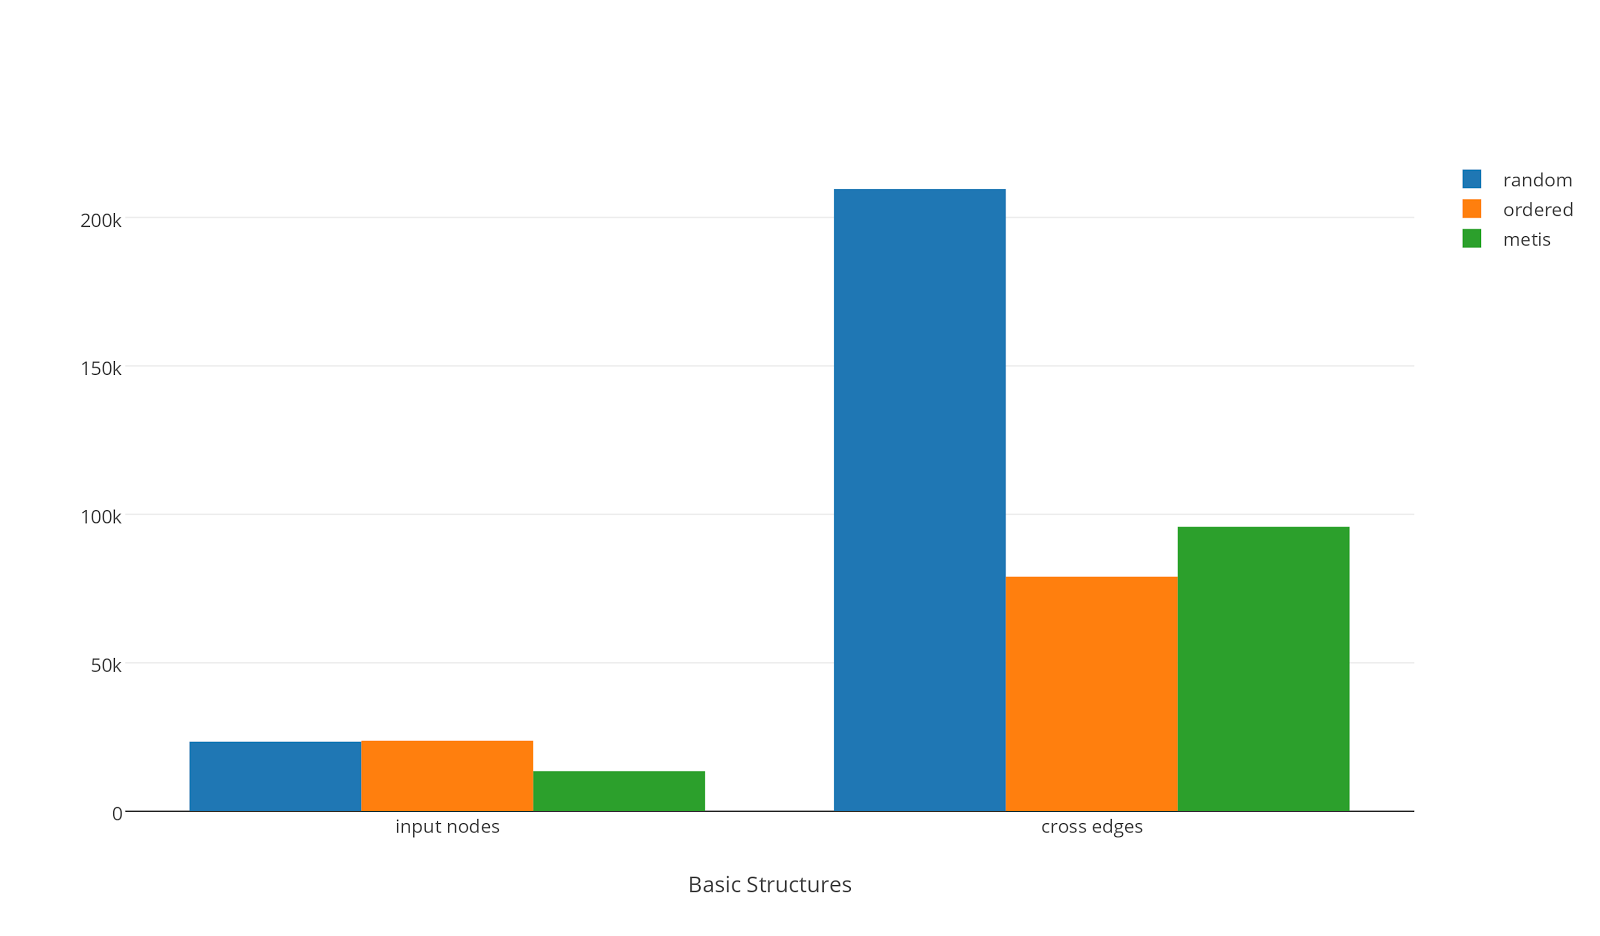
\includegraphics[width=0.8\textwidth]{img/alibaba-structure}
\end{figure}
\\Another interesting finding is that for some queries, different partitioners do not make a difference in the GAG size. In figure \ref{fig:alibaba-Real-World-Queries}, for 8 queries translated from real world, the size of the GAGs are almost the same for different partitioners.
\begin{figure}[h!]
  \caption{GAG Size of Real World Queries}
  \label{fig:alibaba-Real-World-Queries}
  \centering
    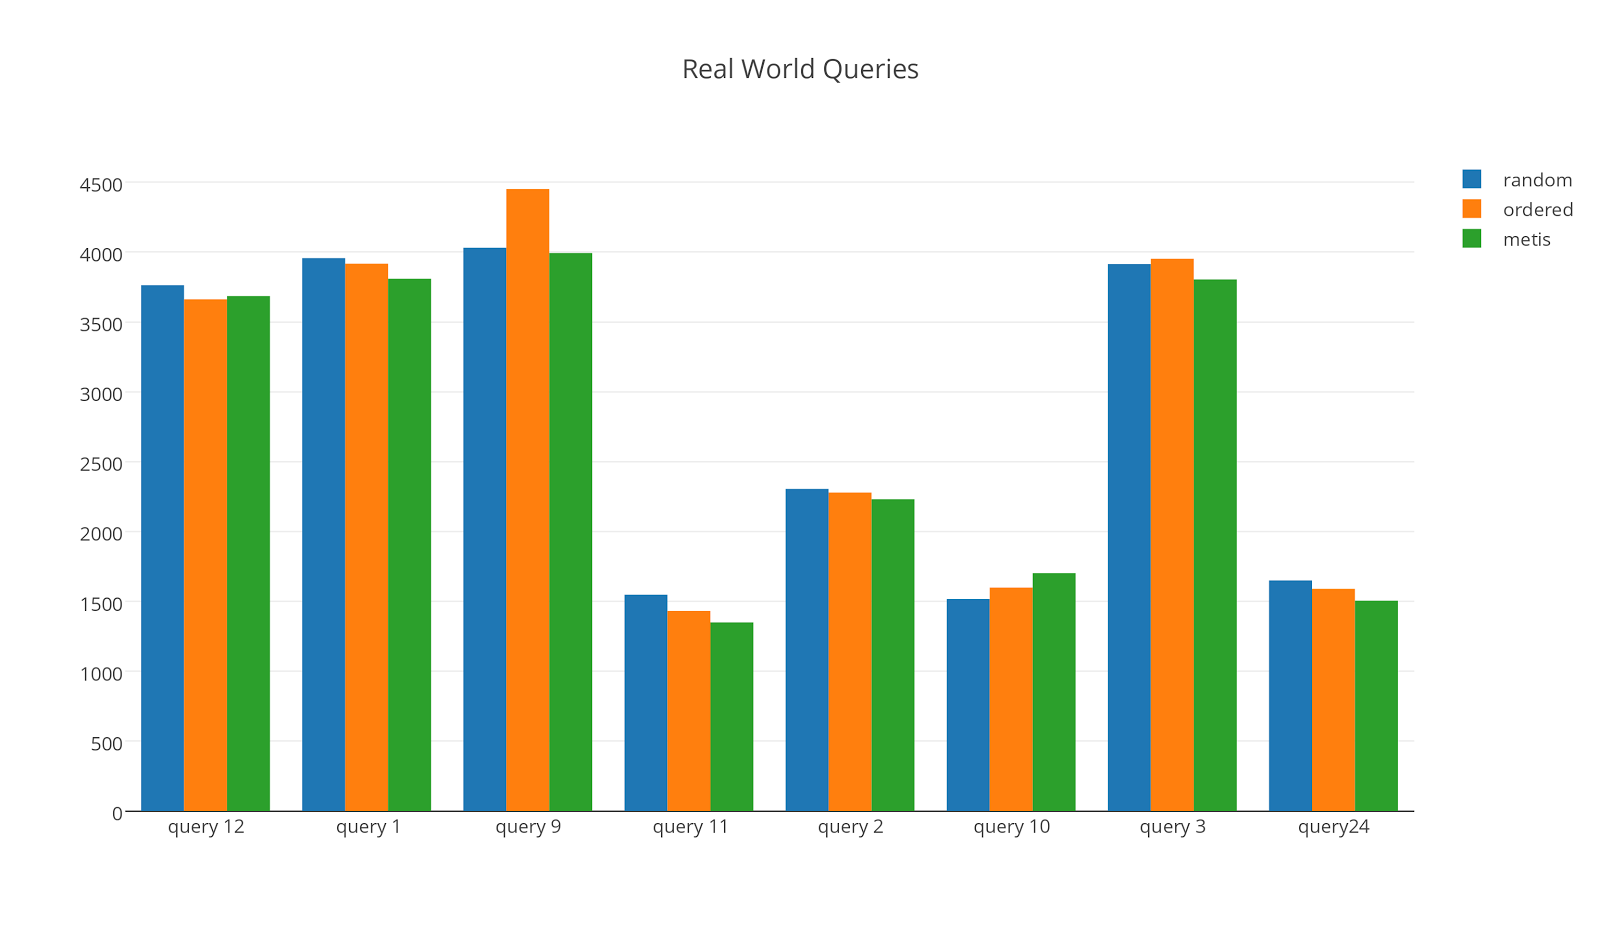
\includegraphics[width=0.8\textwidth]{img/alibaba-Real-World-Queries}
\end{figure}
\\In order to analyze those phenomena, the theoretical size of GAG is analyzed in the next section.
\section{Theoretical Size of GAG}
Recall that the communication cost of the original Dan Suciu's Algorithm is $O(n^2)+O(r)$, where $O(n^2)$ is the size of GAG and $O(r)$ is the size of the result. Actually, the $O(n^2)$ is not always accurate and Dan Suciu gives an  assumption behind it, which we explain in the following.
\\Assuming there are $IN$ input-nodes and $ON$ output-nodes in the distributed graph, then in worst cases, there are $IN*ON*|S|^2$ pairs return to driver side. The assumption behind Dan Suciu's model is that for every input-node there's only one incoming cross-edge, and for each output-node, there's exactly one out cross-edge. Then we can safely conclude that the upper bound of the GAG size is $O(n^2)$.
\\However, in reality not every graph satisfies the model. There can be multiple in-coming cross-edges for one input-node, and multiple out-going cross-edges for one output-node, just like in figure \ref{fig:Cross-Edges}(b), between Dan Suciu's model and fully connected model. Under this model, with a known number of cross-edges, the number of input-nodes can be very different. So we have to focus on algorithms that work with the number of input-nodes now.
\begin{figure}[h!]
  \caption{Different Situations for Cross-Edges}
  \label{fig:Cross-Edges}
  \centering
    \includegraphics[width=0.8\textwidth]{img/Cross-Edges}
\end{figure}
\\So if we extend the case to modified Dan Suciu's Algorithm, the size of GAG, which is also the total communication cost expression, would be:
$$\sum_{\alpha}{(IN_{\alpha}*(|S|-1)+SN_{\alpha})*(ON_{\alpha}*(|S|-1)+FN_{\alpha})}$$
where $IN$ is the number of input-nodes in each site, $|S|$ is the number of states in the automaton, $SN$ is the starting nodes in each site which have out-going edges with same labels as in automata's starting edges, $ON$ is the number of output nodes in each site and $FN$ is the number of nodes where the searching process reaches final states at each site. By the definition of epsilon edges, each output-node in site $\alpha$ has one-on-one relation with one input-node in another site. Then the expression of communication cost would look like:
$$\sum_{\alpha}{(IN_{\alpha}*(|S|-1)+SN_{\alpha})*(\sum_{\beta}{IN_{\beta}}*(|S|-1)+FN_{\alpha})}$$
where $\sum_{\beta}{IN_{\beta}}$ the sum of some input-nodes which connected by epsilon edges from site  $\alpha$.
\\As we start searching from input-nodes and starting-nodes, it's crucial to control their numbers. Generally speaking, for a specific query, $SN$ and $FN$ are fixed, leaving $IN$ the only choice to improve. The expression also explains the phenomenon in figure \ref{fig:alibaba-Real-World-Queries}: For real-world queries whose labels are all rare, $IN*|S|$ is not dominant to $SN$. However, for those queries in figure \ref{fig:alibaba-Random-Queries}, the $SN$ is relatively small, and all labels of non-starting edges in the automaton are quite frequent. Then reducing  $IN$ can improve the performance.
\section{JabeJa Algorithm}
Algorithms 4 and 5 are core parts of the JabeJa Algorithm. At first, each node would be given a color representing its partition. In each round of Algorithm 4, every node $p$ tries to find the best partner which it can swap color with. It communicates with all neighbors first, and if there's no node it can swap color with, it will communicate with a specific random node in the graph. In the end the $p$ exchanges color with its best partner. During the process, simulated-annealing is used to avoid getting stuck in a local optimum and every time a node swaps color successfully, the temperature decreases.
\begin{algorithm}
    \SetKwFunction{proc}{SAMPLEANDSWAP}
    \SetKwProg{myproc}{procedure}{}{endprocedure}
    Require: Any node p in the graph has the following methods:
    \begin{itemize}
        \item $getNeighbors()$: return $p$'s neightbors.
        \item $getRandomSample()$: returns a uniform sample of all the nodes.
        \item $T_0$: the initial temperature.
        \item $\theta$: the cool down speed.
        \item $T_r = T_0$ initially.
    \end{itemize}
    \myproc{\proc{}}{
        \everypar={\nl}
        $partner\leftarrow findPartner(p.getNeighbors(),Tr)$\;
        \If{$partner == null$}{
            $partner \leftarrow findPartner(p.getRandomSample(),Tr)$\;
        }
        \If{$partner \neq null$}{
            handshake for color exchange between $p$ and $partner$\;
        }
        $T_r\leftarrow T_r-\theta$\;
        \If{$T_r<1$}{
            $T_r\leftarrow 1$\;
        }
    }
    \caption{Sample and Swap algorithm at node $p$}
\end{algorithm}
Algorithm 5 describes the way to find the best swap partner. Every time for a node $q$ which $p$ is communicating with, we calculate the degrees of both nodes before and after the swap. If swapping color can decrease the total sum of degrees, it will be compared with the best previous result. In the end, the best partner is returned. The actual swapping operation is implemented as an optimistic transaction, which indicates that the actual swap is done after the two nodes perform a handshake and agree on the swap.
\begin{algorithm}
    \SetKwFunction{proc}{FINDPARTNER}
    \SetKwProg{myproc}{function}{}{endfunction}
    Require: Any node p in the graph has the following methods:
    \begin{itemize}
        \item $getDegree(c)$: return the number of $p$'s neighbors that have color $c$.
    \end{itemize}
    \myproc{\proc{$Node[] \; nodes, float \; T_r$}}{
        \everypar={\nl}
        $highest \leftarrow 0$\;
        $bestPartner \leftarrow null$\;
        \For{$q \in nodes$}{
            $x_{pp} \leftarrow p.getDegree(p.color)$\;
            $x_{qq} \leftarrow q.getDegree(q.color)$\;
            $old \leftarrow x_{pp}+x_{qq}$\;
            
            $x_{pq} \leftarrow p.getDegree(q.color)$\;
            $x_{qp} \leftarrow q.getDegree(p.color)$\;
            $new \leftarrow x_{pq}+x_{qp}$\;
            
            \If{$ (new \times T_r > old) \wedge (new > highest) $ }{
                $bestPartner \leftarrow q$\;
                $highest \leftarrow new$\;
            }
        }
        \Return{$bestPartner$}
    }
    \caption{Find the best node as swap partner for node $p$}
\end{algorithm}
\section{Modified JabeJa Algorithm}
Algorithm 4 remains the same in modified JabeJa algorithm. To minimize the total number of input-nodes in the graph, we  modify the $findPartner$ function, which decreases the number of cross-edges. Algorithm 6 describes the process of finding the best swap partner that reduces the number of input-nodes for a node $p$. The $nodes$ in input parameters is a set of nodes which have different colors from $p$. For every $q$, we call the $CALCDIFF$ function twice to check if swapping color can decrease the number of input-nodes in neighbors of $p$ and $q$. The $CALCDIFF$ function takes two input-nodes $p$ and $q$ and calculates how many nodes in $p$'s neighborhood will turn into input-nodes, and how many input-nodes would turn from input-nodes to an entirely local node. The returning result is a pair $(pinc, pdec)$, which represents the increase and decrease number of input-nodes respectively.
\begin{algorithm}
    \SetKwFunction{proc}{FINDPARTNER}
    \SetKwFunction{calcdiff}{CALCDIFF}
    \SetKwProg{myproc}{function}{}{endfunction}
    \SetKwProg{mycalcdiff}{function}{}{endfunction}
    Require: Any node p in the graph has the following methods:
    \begin{itemize}
        \item $getInDegree()$: return number of $p$'s in-neighbors.
        \item $getInDegree(c)$: return number of $p$'s in-neighbors that have color $c$.
        \item $isInputNode()$: check if $p$ is an input-node.
        \item $getOutNeighbors()$: return $p$'s out-neighbors.
    \end{itemize}
    \myproc{\proc{$Node[] \; nodes, float \; T_r$}}{
        \everypar={\nl}
        $highest \leftarrow 0$\;
        $bestPartner \leftarrow null$\;
        \For{$q \in nodes$}{
            $(pinc,pdec) = CALCDIFF(p,q)$\;
            $(qinc,qdec) = CALCDIFF(q,p)$\;
            $old \leftarrow pinc+qinc$\;
            $new \leftarrow pdec+qdec$\;
            \If{$ (new \times T_r > old) \wedge (new > highest) $ }{
                $bestPartner \leftarrow q$\;
                $highest \leftarrow new$\;
            }
        }
        \Return{$bestPartner$}
    }
    \mycalcdiff{\calcdiff{$Node \; p, Node \; q$}}{
        \everypar={\nl}
        $pNeighbors \leftarrow p.getOutNeighbors()\backslash q.getOutNeighbors()\backslash \{q\}$\;
        $pinc \leftarrow 0$\;
        $pdec \leftarrow 0$\;
        \For{$k \in pNeighbors$}{
            \If{$k.isInputNode() = false$}{
                $pinc \leftarrow pinc + 1$\;
            }
            \If{$k.getInDegree(k.color) = k.getInDegree()-1 \wedge q.color = k.color$}{
                $pdec \leftarrow pdec + 1$\;
            }
        }
        \If{$p \notin q.getOutNeighbors() \wedge p.getInDegrees()>0$ }{
            \If{$p.isInputNode() = false$}{
                $pinc \leftarrow pinc + 1$\;
            }
            \ElseIf{$p.getInDegree(q.color) = p.getInDegree()$}{
                $pdec \leftarrow pdec + 1$
            }
        }
        \Return{$(pinc,pdec)$}
    }
    \caption{Find the best swap partner that minimize \#$inputnodes$ for node $p$}
\end{algorithm}
\\The body of function $CALCDIFF$ can be explained with the help of figure \ref{fig:modified-dan-example}, here we call nodes that are not input-nodes local-nodes.
\\Line 15-16 initialize the increase and decrease number of input-nodes to be 0.
\\Line 14 ensures that nodes which are out-neighbors of both $p$ and $q$, get ignored since swapping color would not change the node status (Figure \ref{fig:modified-dan-example}(a)). At the same time, $q$ is a special case and needs to be considered separately. 
\\Line 17-24 explains the process of examining the status of each node in $pNeighbors$: 
\begin{enumerate}
    \item If it's currently not a input-node, then after swapping it would definitely be a input-node since new color of $p$ is different (Figure \ref{fig:modified-dan-example}(b)).
    \item If it's currently a input-node, has same color with $q$ and $p$ is the only node with different color, then current node will turn from input-node to a local-node (Figure \ref{fig:modified-dan-example}(c)).
\end{enumerate} 
Line 25-31 explains the process of examining the status of $p$:
\begin{enumerate}
    \item If $p$ is one of $q$'s neighbors or its in-degree is 0, swapping color would makes no difference for $p$'s status.
    \item If $p$ is not a input-nodes, swapping color would make it becomes a input-node (Figure \ref{fig:modified-dan-example}(d)).
    \item If all of $p$'s has same number of in-neighbors of $q$'s color as in-degree, swapping color turns $p$ from input-node to a local-node (Figure \ref{fig:modified-dan-example}(e)).
\end{enumerate}
\begin{figure}[h!]
  \caption{Different Situations for Examining Input-Nodes}
  \label{fig:modified-dan-example}
  \centering
    \includegraphics[width=1.0\textwidth]{img/modified-dan-example}
\end{figure}
In theory, the more nodes $p$ tries to swap with in every iteration, the larger the chance is that it goes to the best result. If every time $p$ communicates with all other nodes in graph, it would choose the best swap partner in theory, even if it's very time-consuming. So in polynomial time  $O(|V|^2)$ a given partitioning situatjion can be checked if it's the best solution, if we assume the $FINDPARTNER$ function takes one unit time.
\section{Evaluation}
Every node in the graph runs Algorithm 4 concurrently. Similar to the Original JabeJa algorithm, the actual swap is done after the two nodes perform a handshake and agree on the swap. As function $getInDegree(c)$ would access shared data which could be updated after a swap, the algorithm should be implemented with an asynchronous programming model. Under this circumstance, Spark is not suitable for implementation. Although there is a simple implementation\cite{jabejagraphchi} of JabeJa algorithm on GraphChi\cite{kyrola2012graphchi}, a disk-based graph computing system based on the asynchronous model, it's still time-consuming to study a new platform and code in a new programming model. We focus on comparing the number of input-nodes, but not the offline performance of the algorithms. So we implemented the modified JabeJa Algorithm sequentially and simulated the result.
\subsection{Approach}
The experiment steps are as followed:
\begin{enumerate}
    \item Generate random graphs and queries with GMark Benchmark. The graphs have $10^5$, $10^6$, and $10^7$ nodes respectively. We stop at $10^7$ as the size of $GAG$ has upper bound $(|V||S|)^2$ and it might be very expensive to compute on the driver for a larger graph.
    \item Check the queries, keep those which start with rare labels and delete those which take longer than 1 hours to solve sequentially.
    \item Run four partition strategies against those graphs with different partition numbers and check the number of input-nodes in each setting. For the METIS algorithm, we use the available library at \cite{metislib}. For JabeJa and modified JabeJa, we use the single-thread program mentioned above.
    \item Use the modified Dan Suciu's algorithm to evaluate random queries in step 2 on top of graphs with different partition strategies, and compare the size of GAG, running time and driver-side computation time for each query.
\end{enumerate}
\subsubsection{Parameter Selection} We set initial temperature $T_0 = 2$ and cool down speed $\theta = 0.01$ in simulated annealing, which is similar to existing implementation in GraphChi. Each iteration the program calls $FINDPARTNER$ for every node. If there are no neighbors to swap with, we choose five random nodes with different colors for it and call $FINDPARTNER$ again. The program terminates when the input-nodes number remains the same for ten iterations.
\subsection{Metrics}
We observed the following:
\begin{enumerate}
    \item Input-Nodes: The main property to investigate. We will try to find out the relation between input-nodes number and running time of the algorithm.
    \item Cross-Edges: When two partition strategies have a close number of input-nodes, the one with fewer cross-edges is preferred as it might be optimal for other kinds of query algorithms in a graph database.
    \item Size of the GAG: The amount of data transmitted in the network. It could also affect the performance on the driver side.
    \item Driver-Computation Time: The computation time after the driver receives GAG. This is investigated for the queries whose evaluation bottleneck is on the driver side.
    \item Overall Running Time: The total time spent on solving each query.
\end{enumerate}

\subsection{Research Questions}
The research questions related to the metrics can be formulated as followed:
\begin{enumerate}
    \item How does JabeJa* perform in minimizing input-node number comparing to other partitioners?
    \item As the input-node number decreases, will the size of GAG decreases?
    \item As the GAG size decreases, will the driver computation time decreases?
    \item As the GAG size decreases, will the overall evaluation time decreases?
\end{enumerate}

\subsection{Input-Nodes and Cross-Edges}
In this part, the number of input-nodes and cross-edges are listed along with the different number of partitions. For the legends, the suffix `ce' is short for cross-edge and `in' is short for input-node. `JabeJa*' represents the modified JabeJa Algorithm. Sometimes the default partitioner is also written as 'ordered' as it's the basic approach of the partitioner.
\subsubsection{Alibaba}
For Benchmark Alibaba, the number of cross-edges and input-nodes are shown in Figure \ref{fig:Alibaba-Partitioners}: Both of the numbers become relatively stable when we divide the graph into 32 partitions. The interesting findings are:
\begin{enumerate}
    \item METIS turns out to be optimal in reducing input-nodes. However, it does not lead to the best number of cross-edges, which the algorithm is developed to optimize initially.
    \item JABEJA beats METIS in the number of cross-edges, but the input-nodes number is still around $50\%$, which is far from the best.
    \item The modified JabeJa Algorithm cuts the number of input-nodes compared to original JabeJa algorithm, but as a trade-off, the number of cross-edges is much worse than with the JabeJa algorithm.
    \item Most of the time, the random and default partitioner are worst in both the number of cross-edges and the number of input-nodes. However, the default partitioner has a good number of cross-edges when there are only a few partitions.
\end{enumerate}
\begin{figure}[h!]
  \caption{Input-node and Cross-edge size of Alibaba Graph}
  \label{fig:Alibaba-Partitioners}
  \centering
    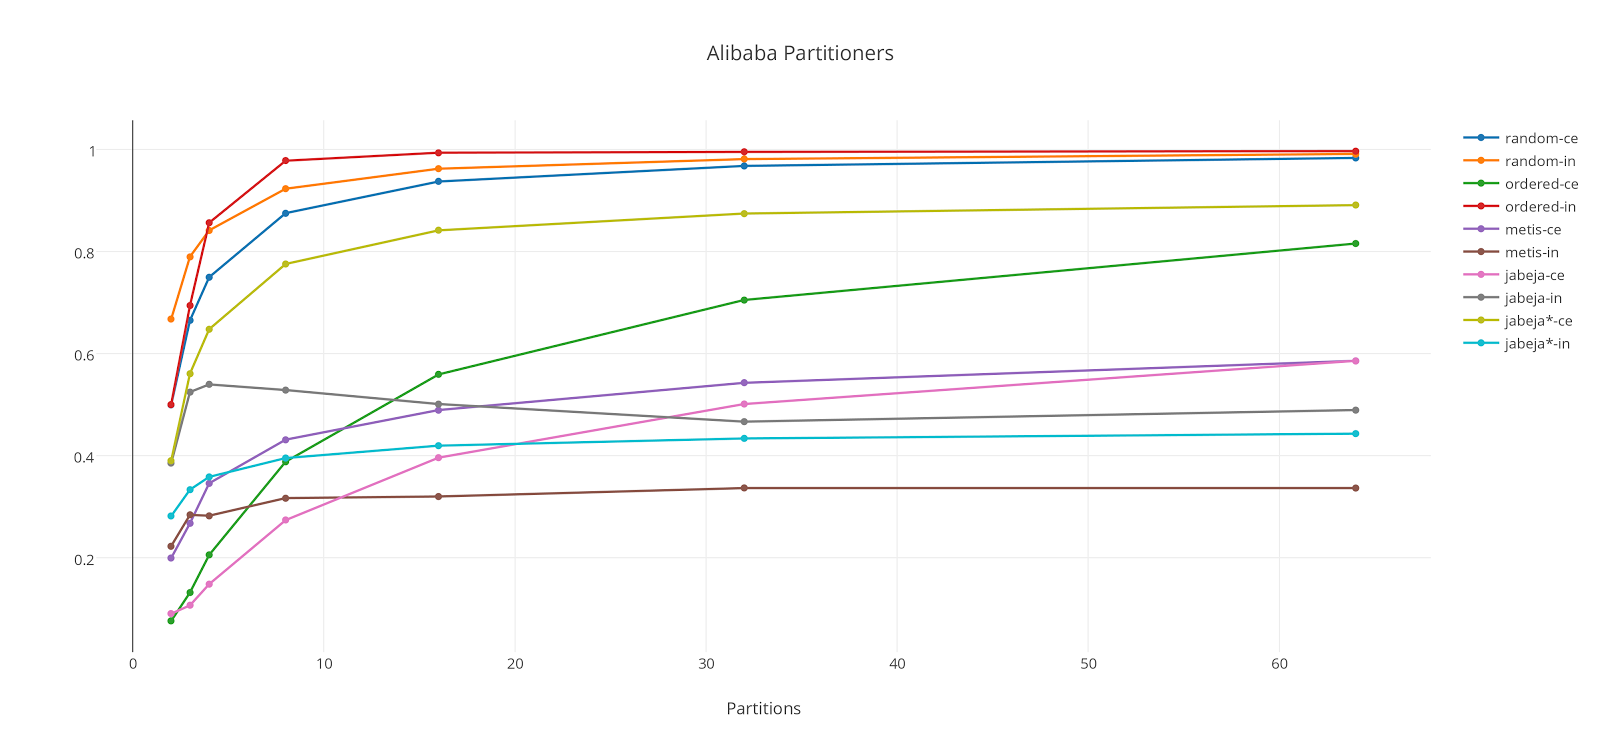
\includegraphics[width=1.0\textwidth]{img/Alibaba-Partitioners}
\end{figure}

\subsubsection{YouTube}
For the YouTube Benchmark, the ratio of cross-edges and input-nodes compared to corresponding total numbers are presented in Figure \ref{fig:Youtube-Partitioners}. The main observations are:
\begin{enumerate}
    \item JabeJa has the least cross-edges and even beats METIS.
    \item JabeJa* has the largest number of cross-edges, which is worse than default-partitioners.
    \item The number of input-nodes for non-default partition strategies are all close to 100\% and don't vary with the increase number of partitions. In this case, default partitioning strategy outperforms the strategies we discussed, which suggests that for a dense graph, those algorithm can barely improve the number of input-nodes.
\end{enumerate}
\begin{figure}[h!]
  \caption{Input-node and Cross-edge size of YouTube Graph}
  \label{fig:Youtube-Partitioners}
  \centering
    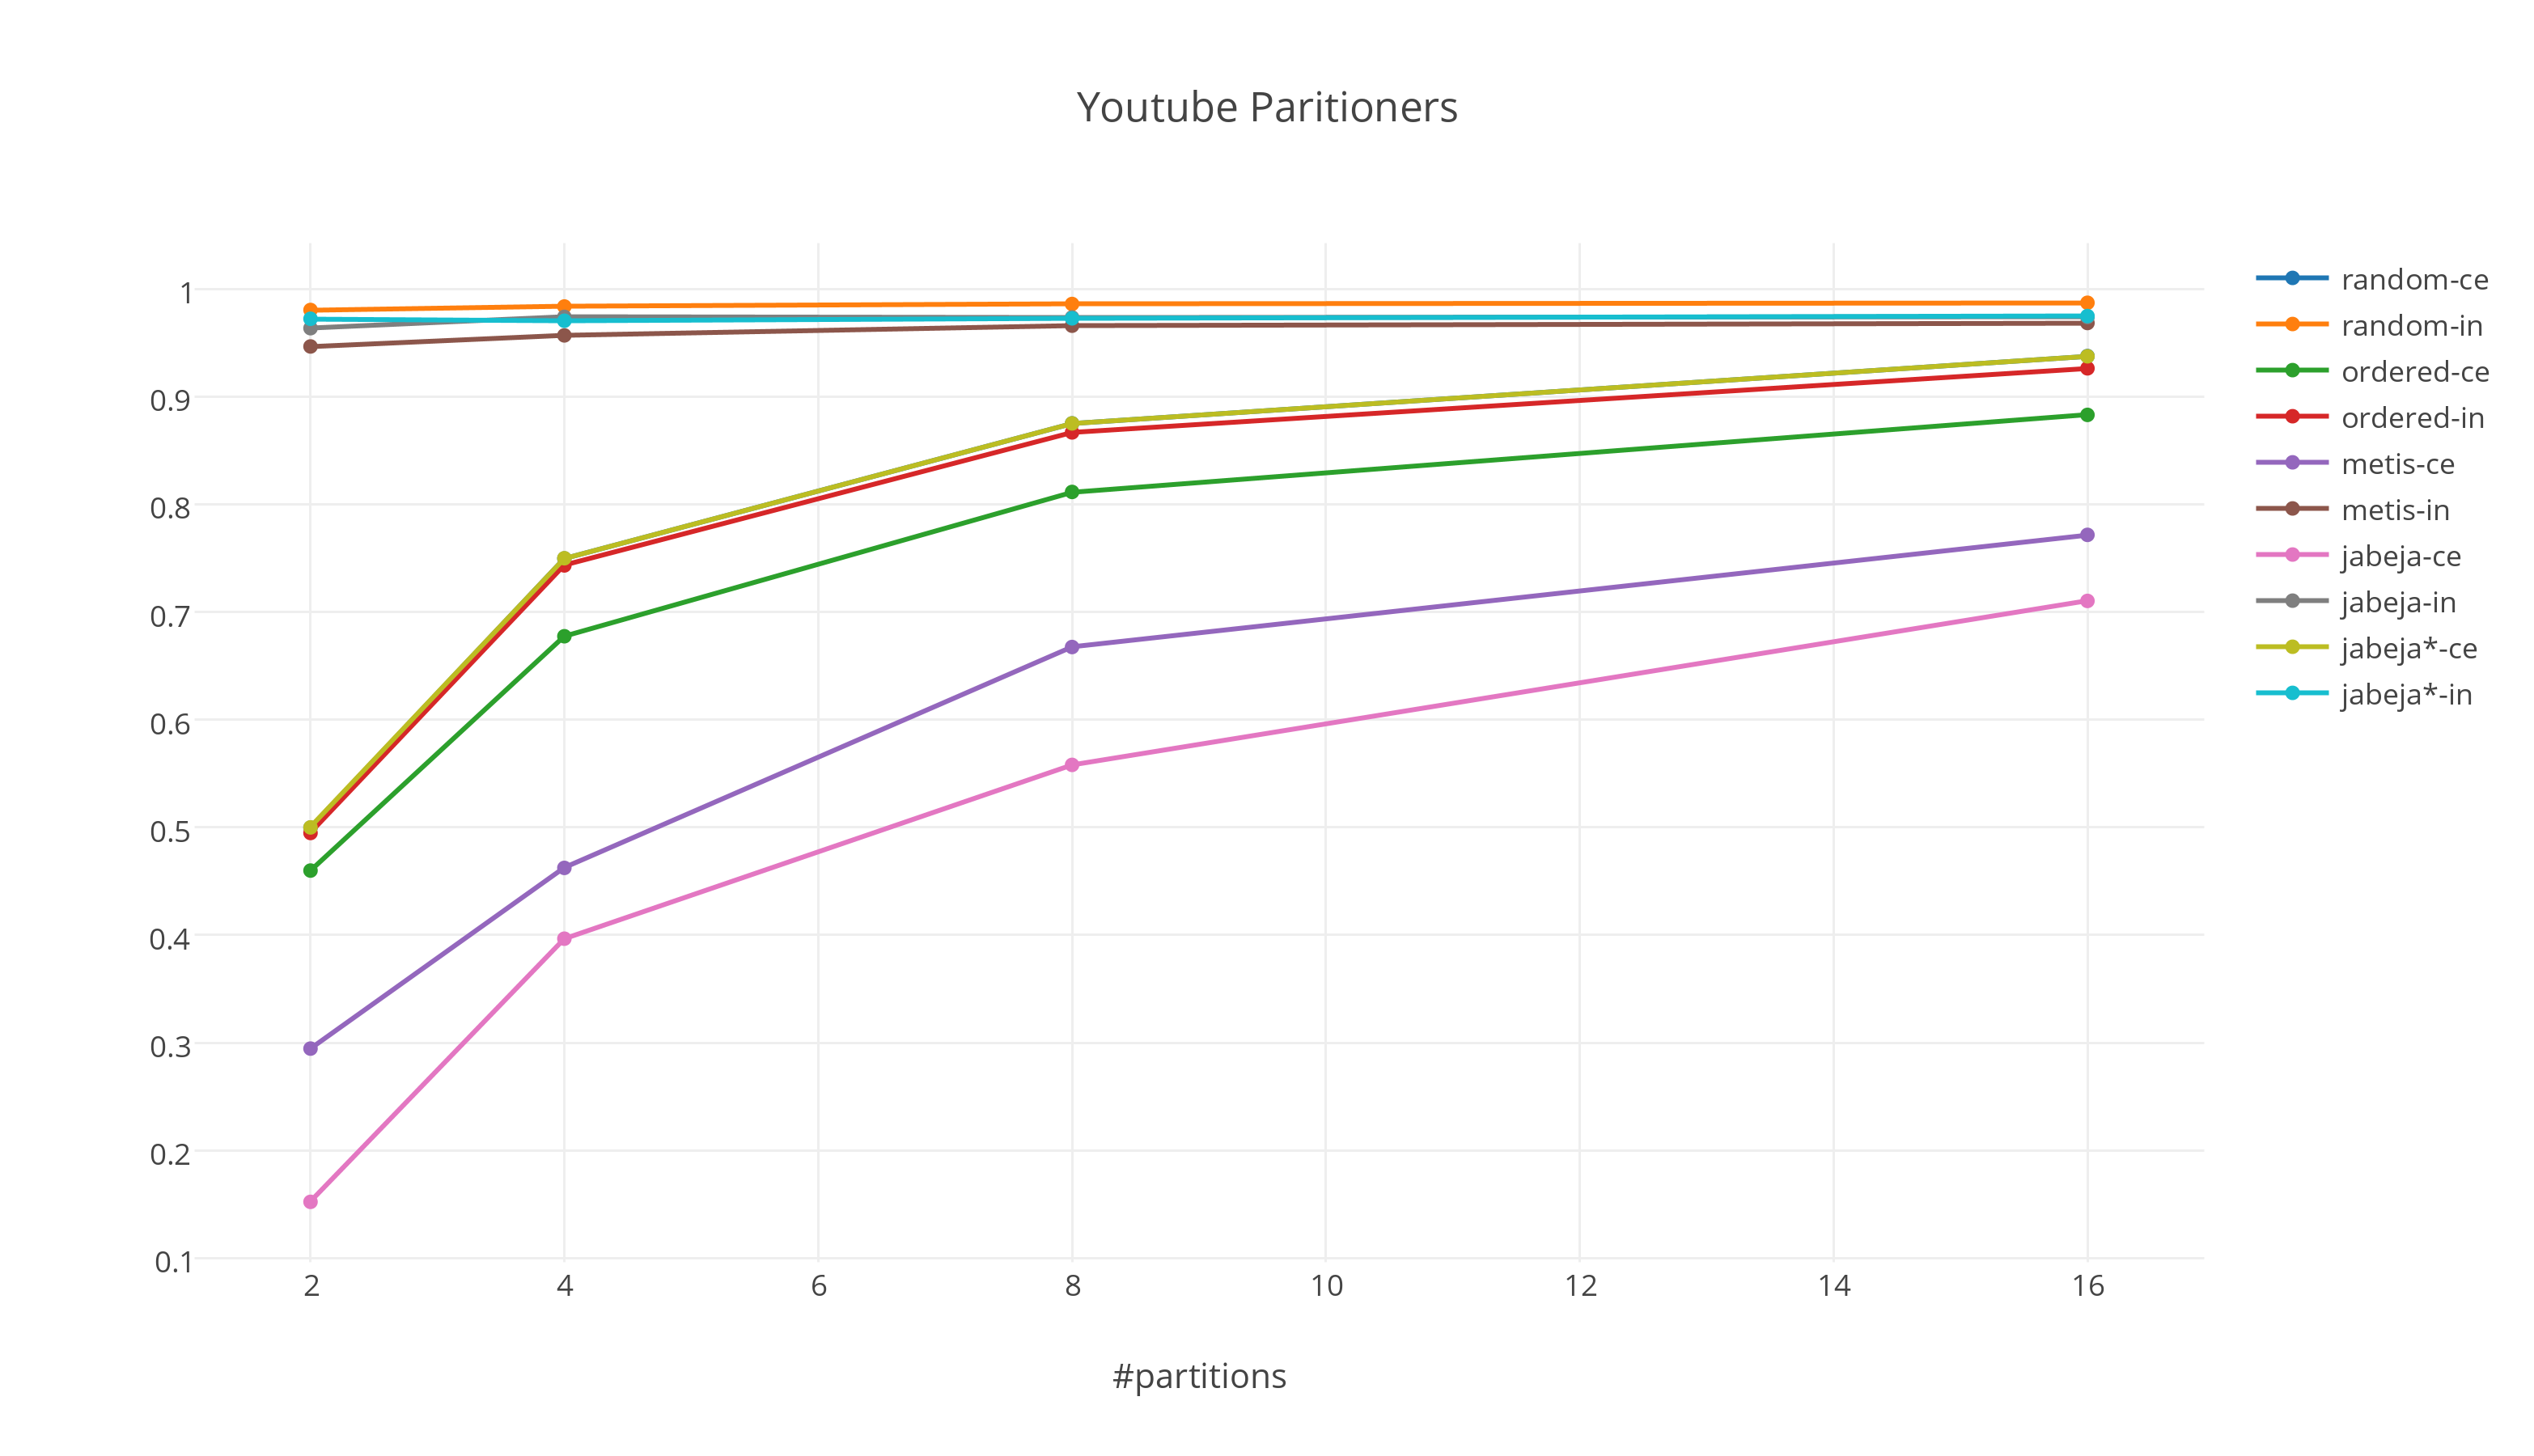
\includegraphics[width=1.0\textwidth]{img/Youtube-Partitioners}
\end{figure}

\subsubsection{Higgs}
For Benchmark Higgs, Figure \ref{fig:Higgs-Partitioners} shows the ratio of cross-edges and input-nodes. The followings are key findings:
\begin{enumerate}
    \item The METIS strategy has the least input-nodes with various numbers of partitions.
    \item JabeJa is slightly better than METIS with regards to cross-edges in the end, and is the best when there are 16 partitions.
    \item JabeJa* is not improving both the numbers of input-nodes and cross-edges.
\end{enumerate}
\begin{figure}[h!]
  \caption{Input-node and Cross-edge size of Higgs Graph}
  \label{fig:Higgs-Partitioners}
  \centering
    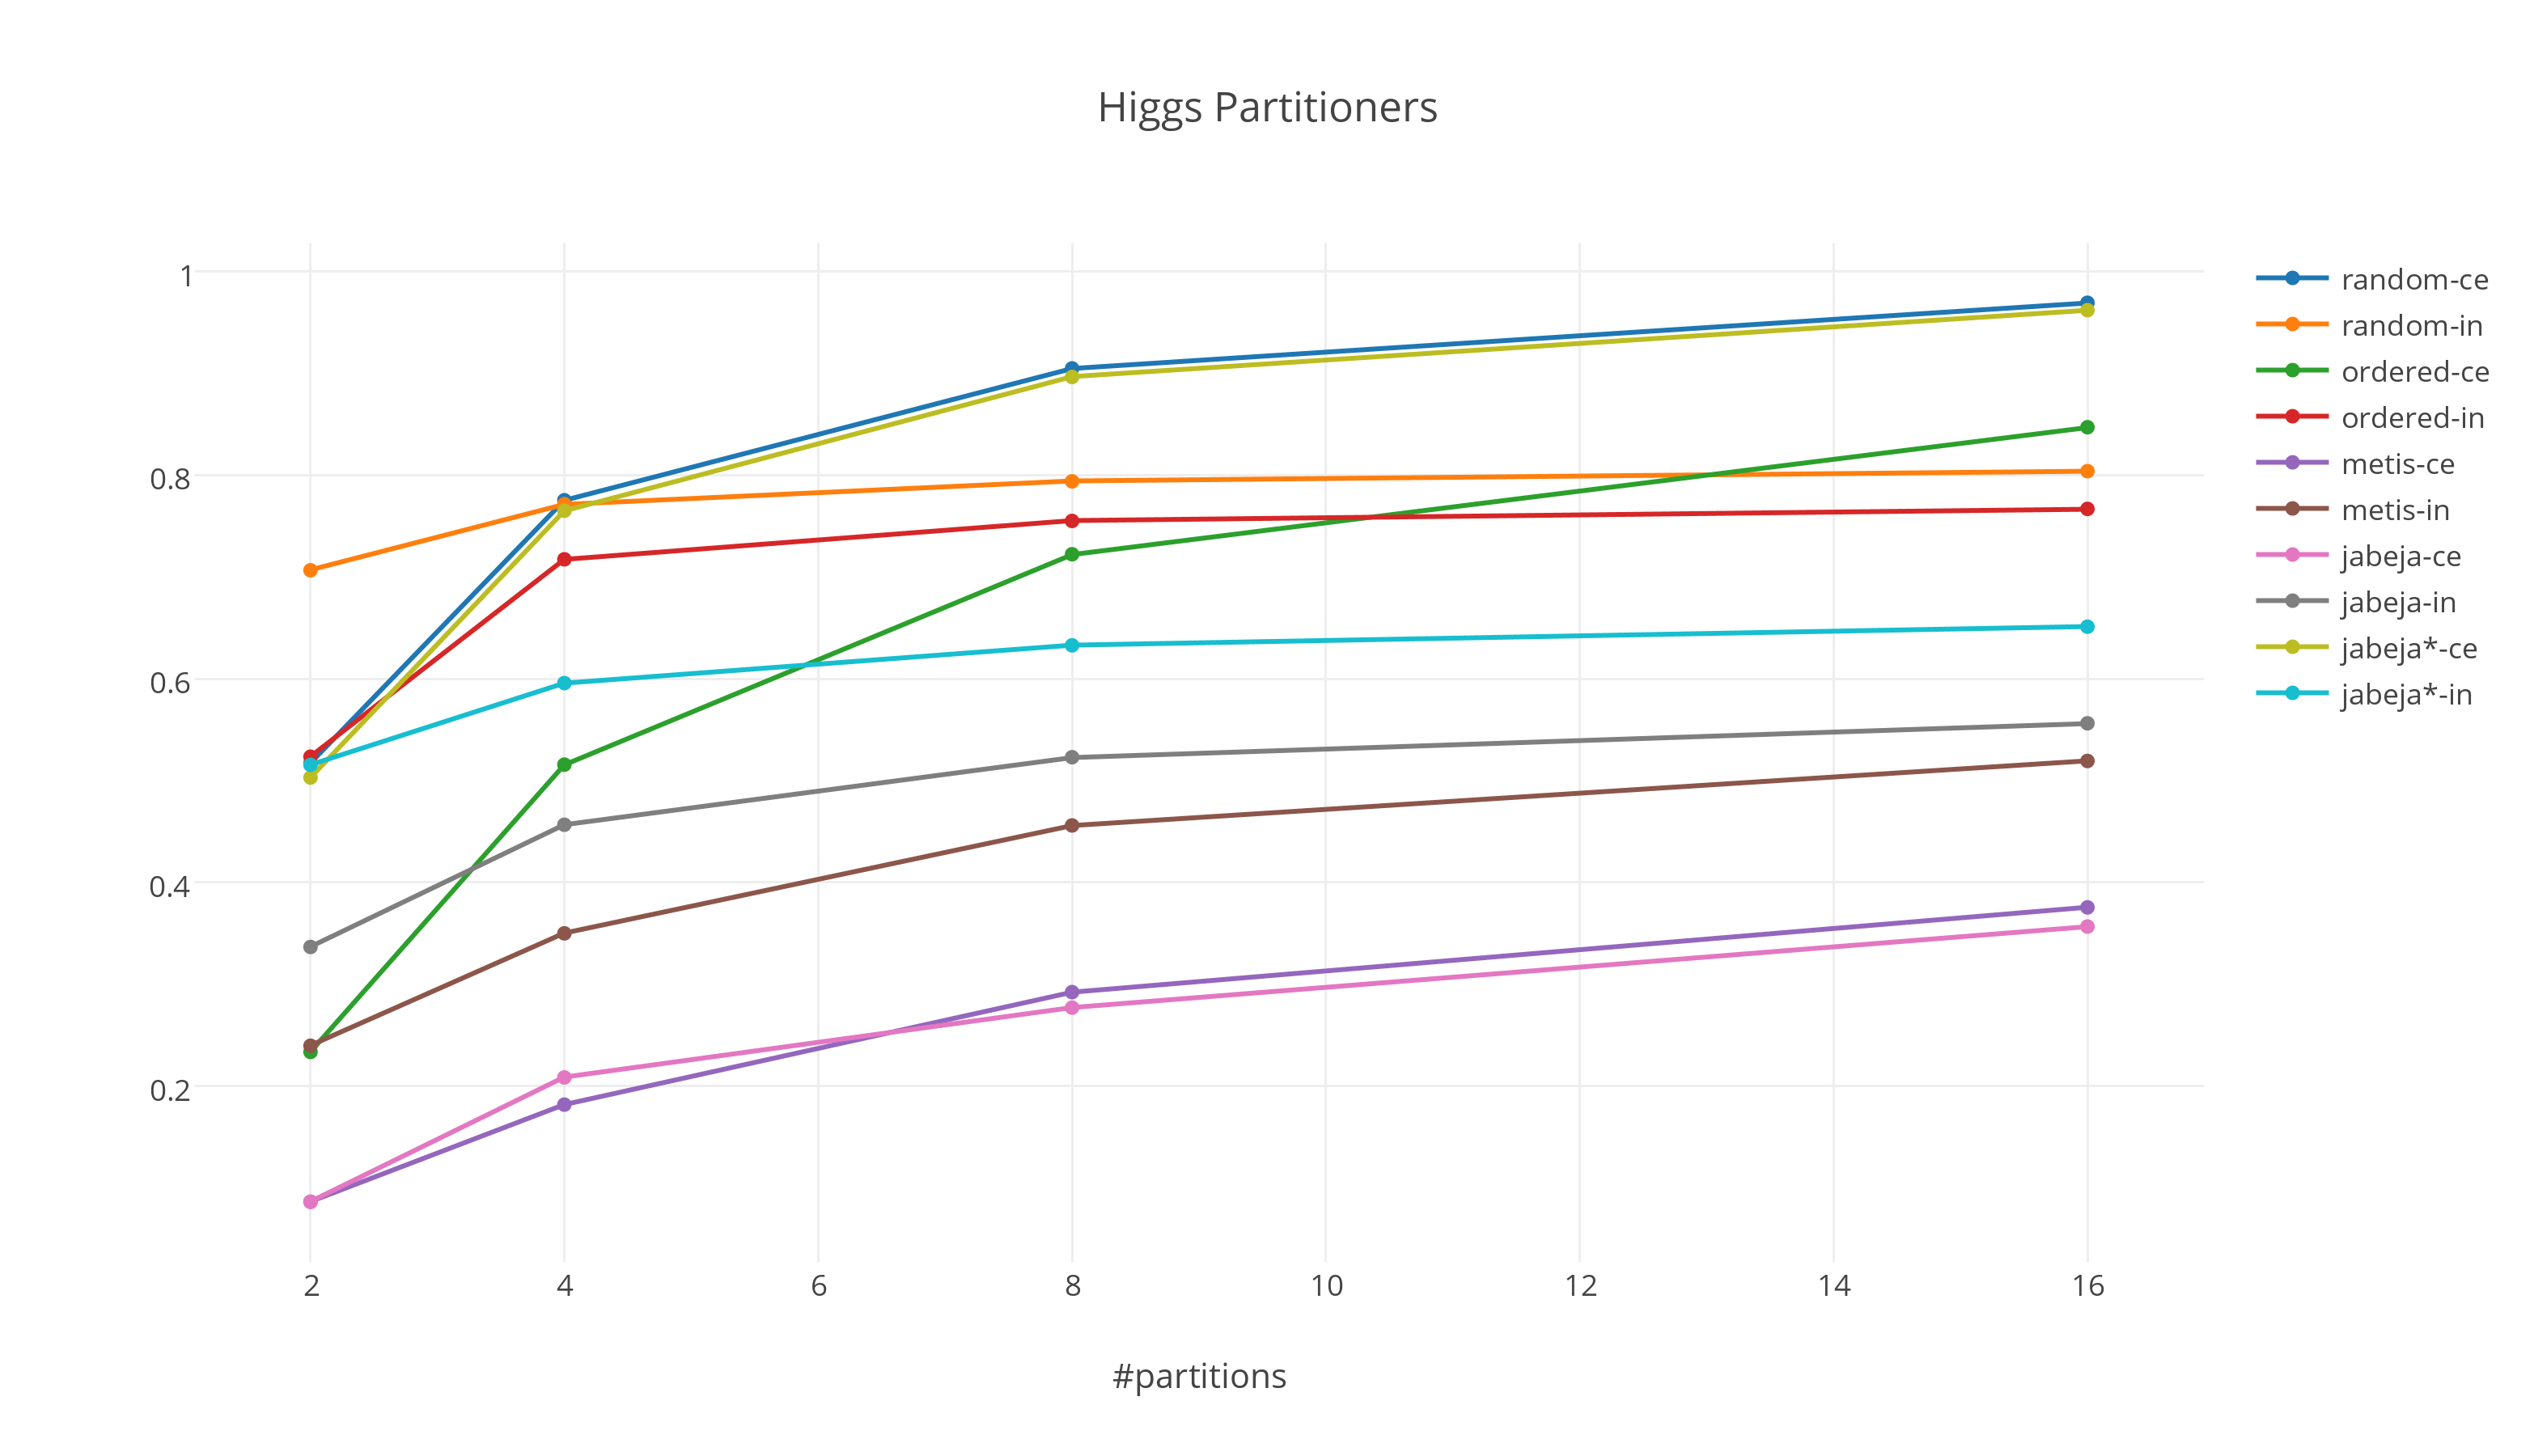
\includegraphics[width=1.0\textwidth]{img/Higgs-Partitioners}
\end{figure}


\subsubsection{GMark Graphs}
We run those partition strategies against three GMark Graphs. The result is as in Figure \ref{fig:0.1m-inputnode}, Figure \ref{fig:1m-inputnode} and Figure \ref{fig:10m-inputnode}. We can see that the three diagrams are almost the same in shape, except the values are multiplied by ten. The number of input-nodes and cross-edges are relatively stable at eight partitions. The interesting findings are:
\begin{enumerate}
    \item This time METIS beats all partition strategies in both input-node and cross-edge number. The number of input-nodes is below $10\%$ of $|V|$, which is an excellent result.
    \item The modified JabeJa Algorithm is slightly better than JabeJa Algorithm concerning with input-node number, but finally they are almost the same when the graph is in 16 partitions.
    \item The default partitioner is worst all the time in input-node and cross-edge numbers. The reason behind it might be that the GMark graphs are randomly generated, unlike Alibaba as a real-world and well-organized benchmark.
\end{enumerate}
\begin{figure}[h!]
  \caption{Input-node and Cross-edge size of GMark Graph ($10^5$ nodes)}
  \label{fig:0.1m-inputnode}
  \centering
    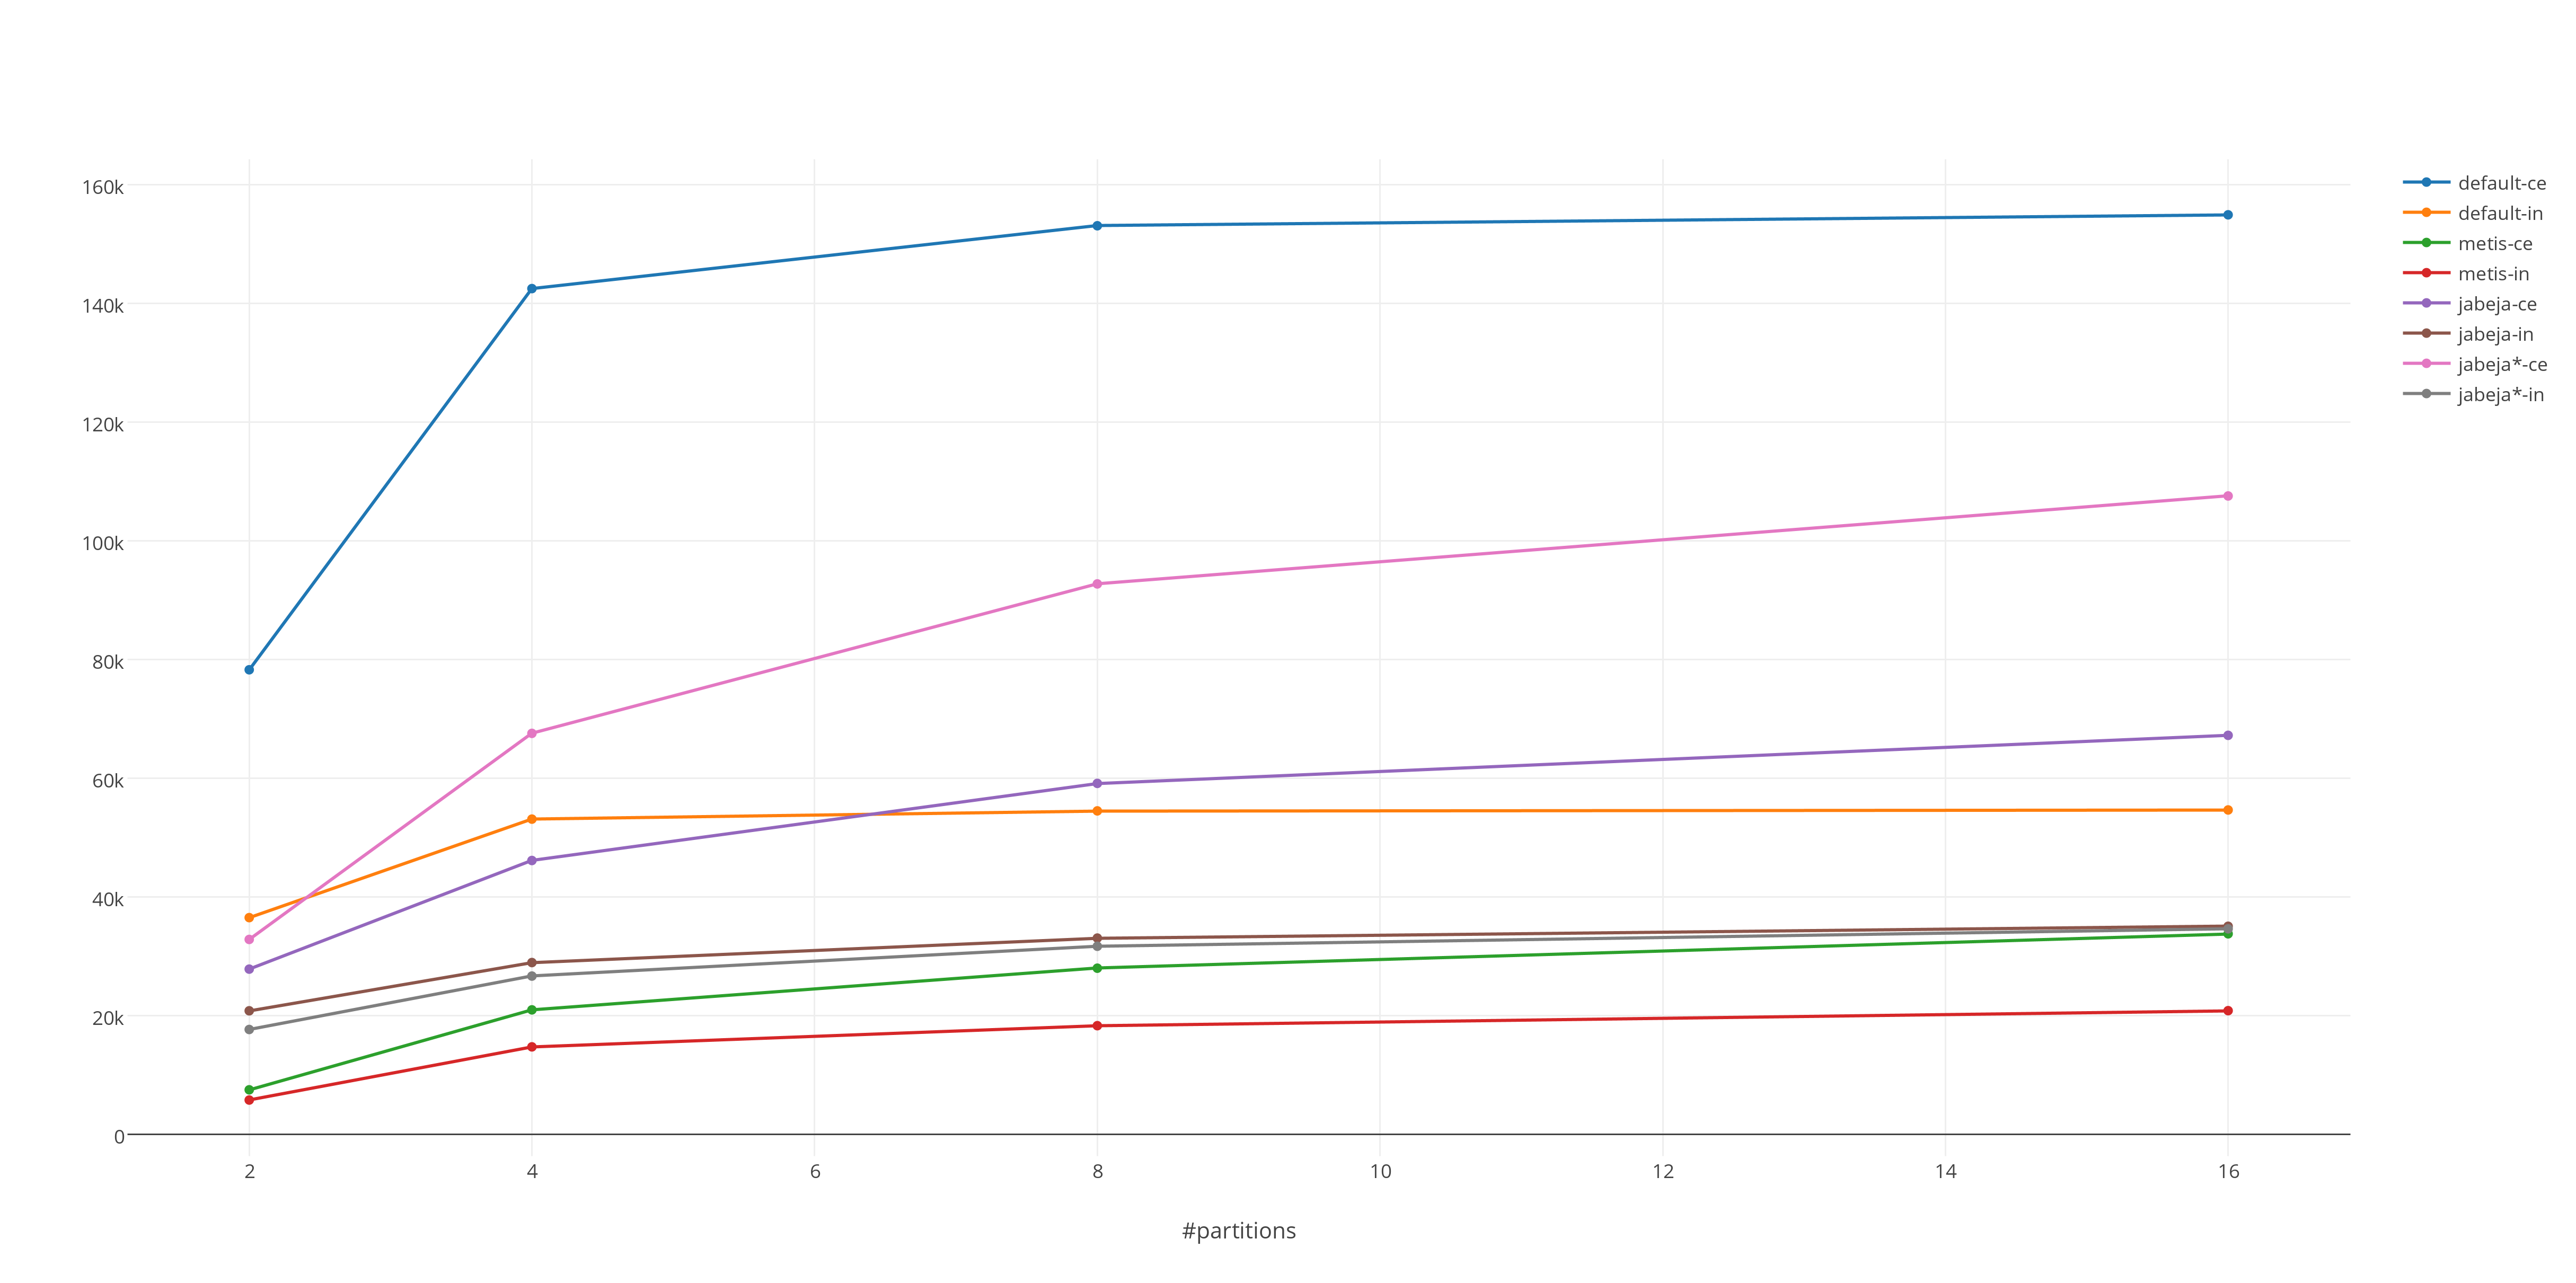
\includegraphics[width=1.0\textwidth]{img/-1m-inputnode}
\end{figure}
\begin{figure}[h!]
  \caption{Input-node and Cross-edge size of GMark Graph ($10^6$ nodes)}
  \label{fig:1m-inputnode}
  \centering
    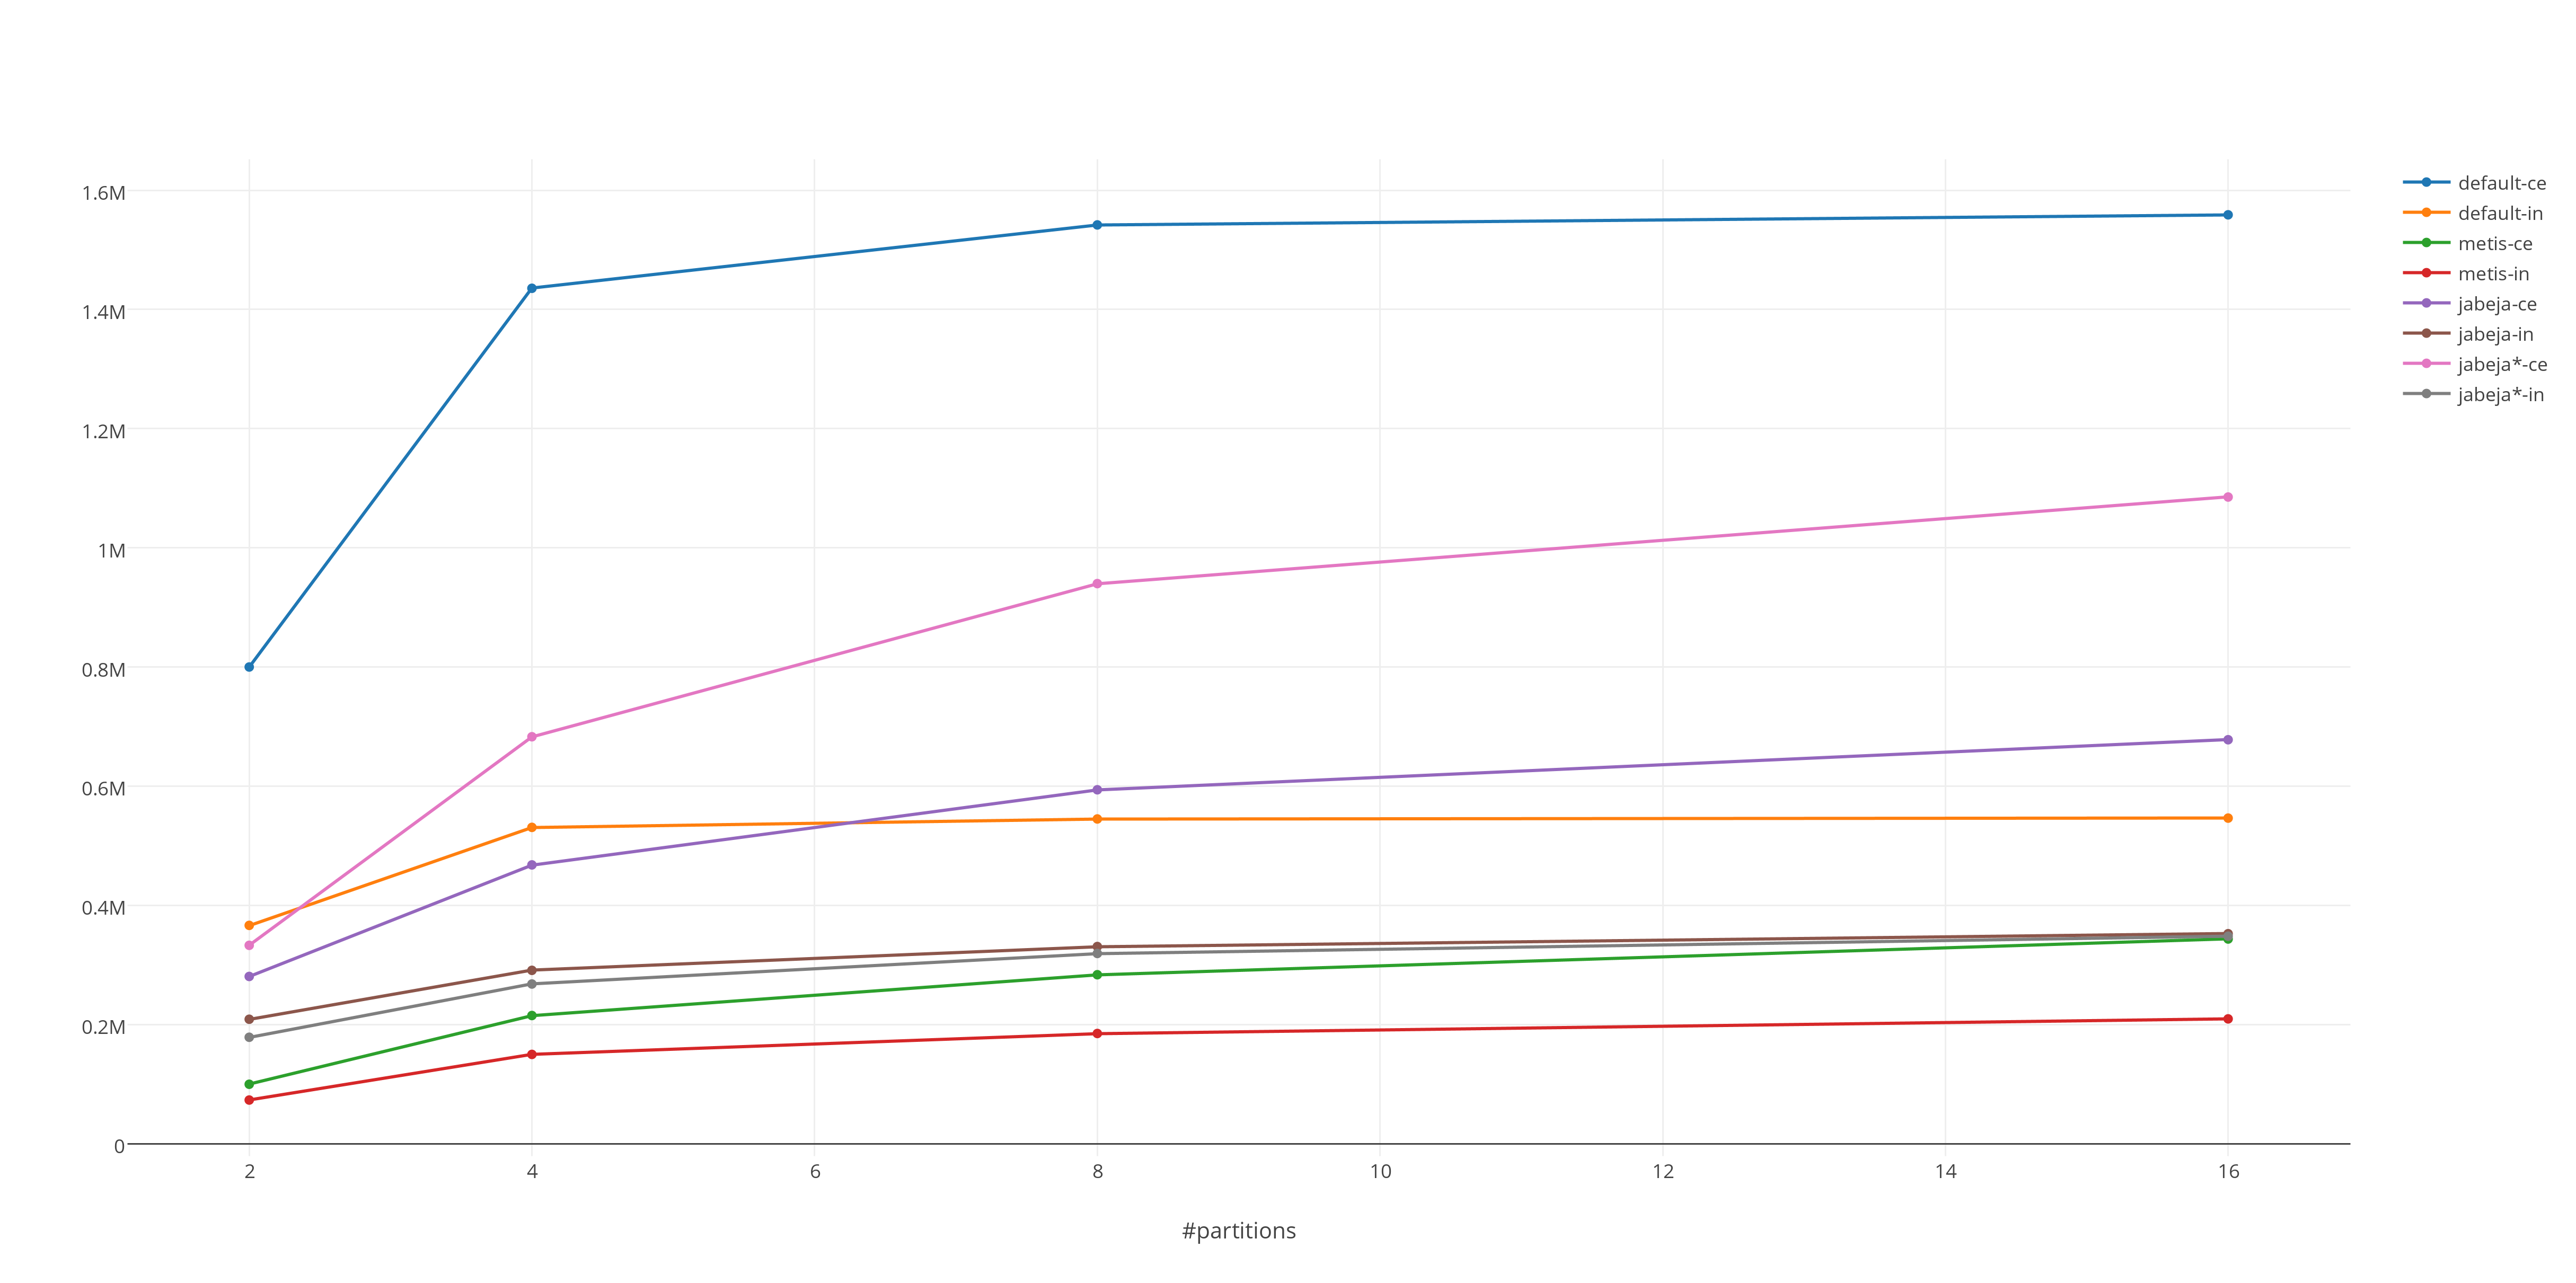
\includegraphics[width=1.0\textwidth]{img/1m-inputnode}
\end{figure}
\begin{figure}[h!]
  \caption{Input-node and Cross-edge size of GMark Graph ($10^7$ nodes)}
  \label{fig:10m-inputnode}
  \centering
    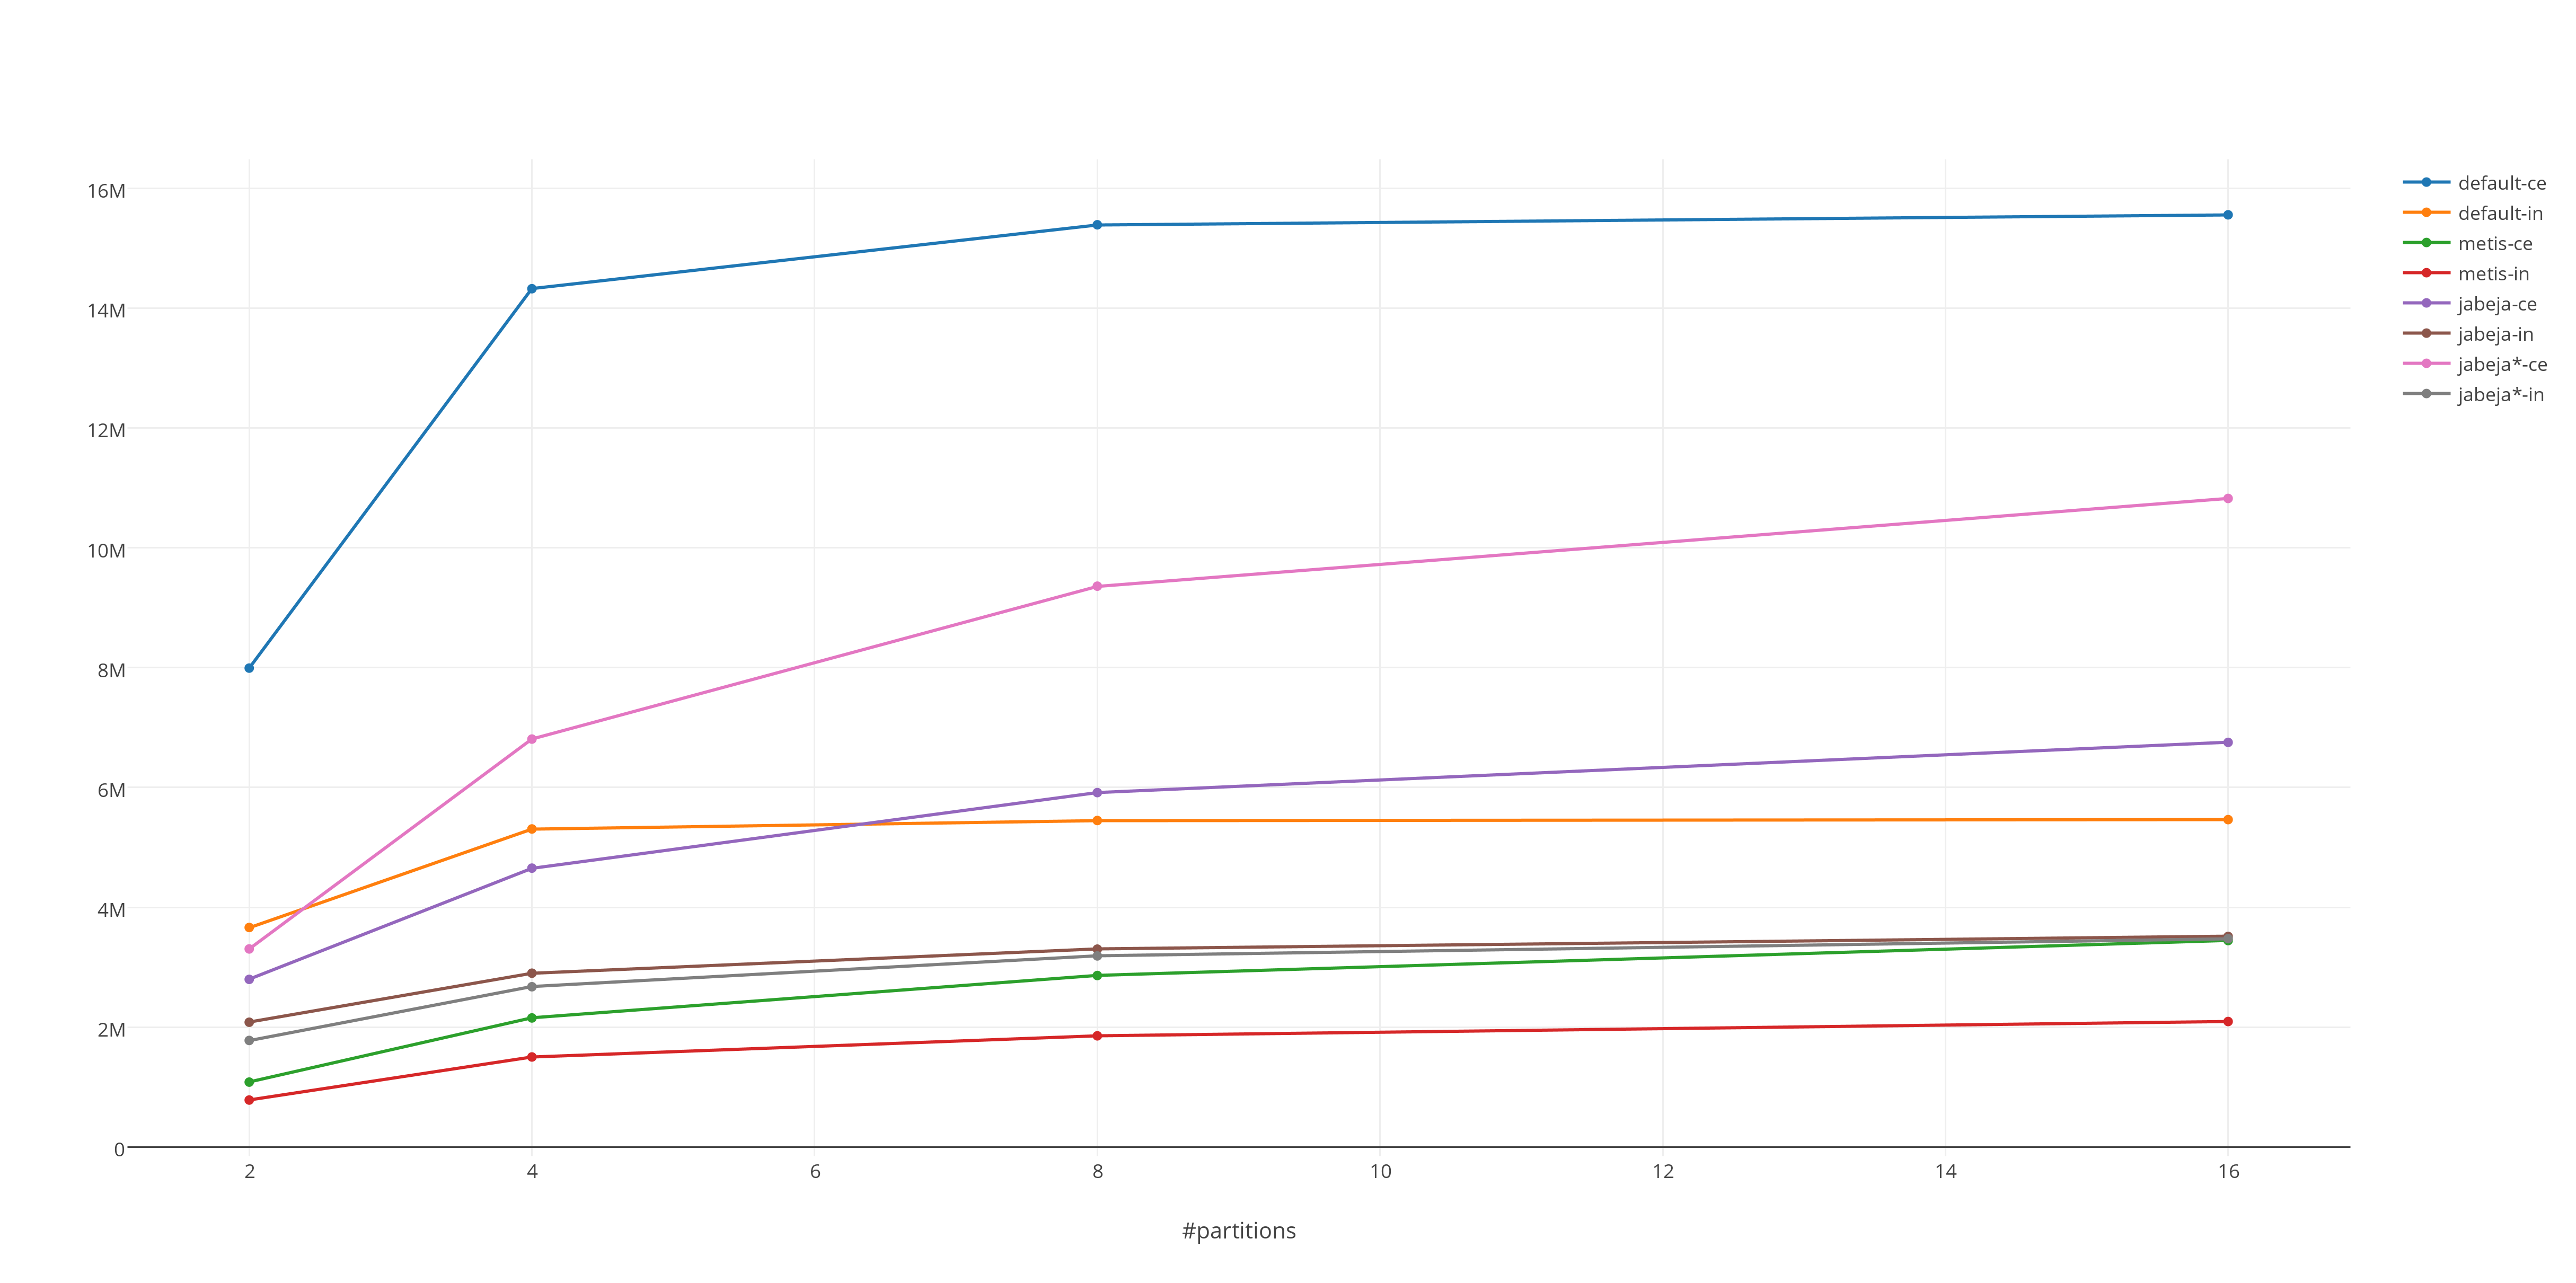
\includegraphics[width=1.0\textwidth]{img/10m-inputnode}
\end{figure}

\subsection{Size of the GAG}
As the number of input-nodes is relatively stable with eight partitions, we run Dan Suciu's Algorithm on GMark graphs split by different strategies with eight workers. The size of GAG can be found in Figure \ref{fig:gmark-01m-gag}, Figure \ref{fig:gmark-1m-gag} and Figure \ref{fig:gmark-10m-gag}. For each query, we list the number of pairs in GAG with different partition strategies.
\begin{figure}[h!]
  \caption{GAG size of GMark Graph ($10^5$ nodes)}
  \label{fig:gmark-01m-gag}
  \centering
    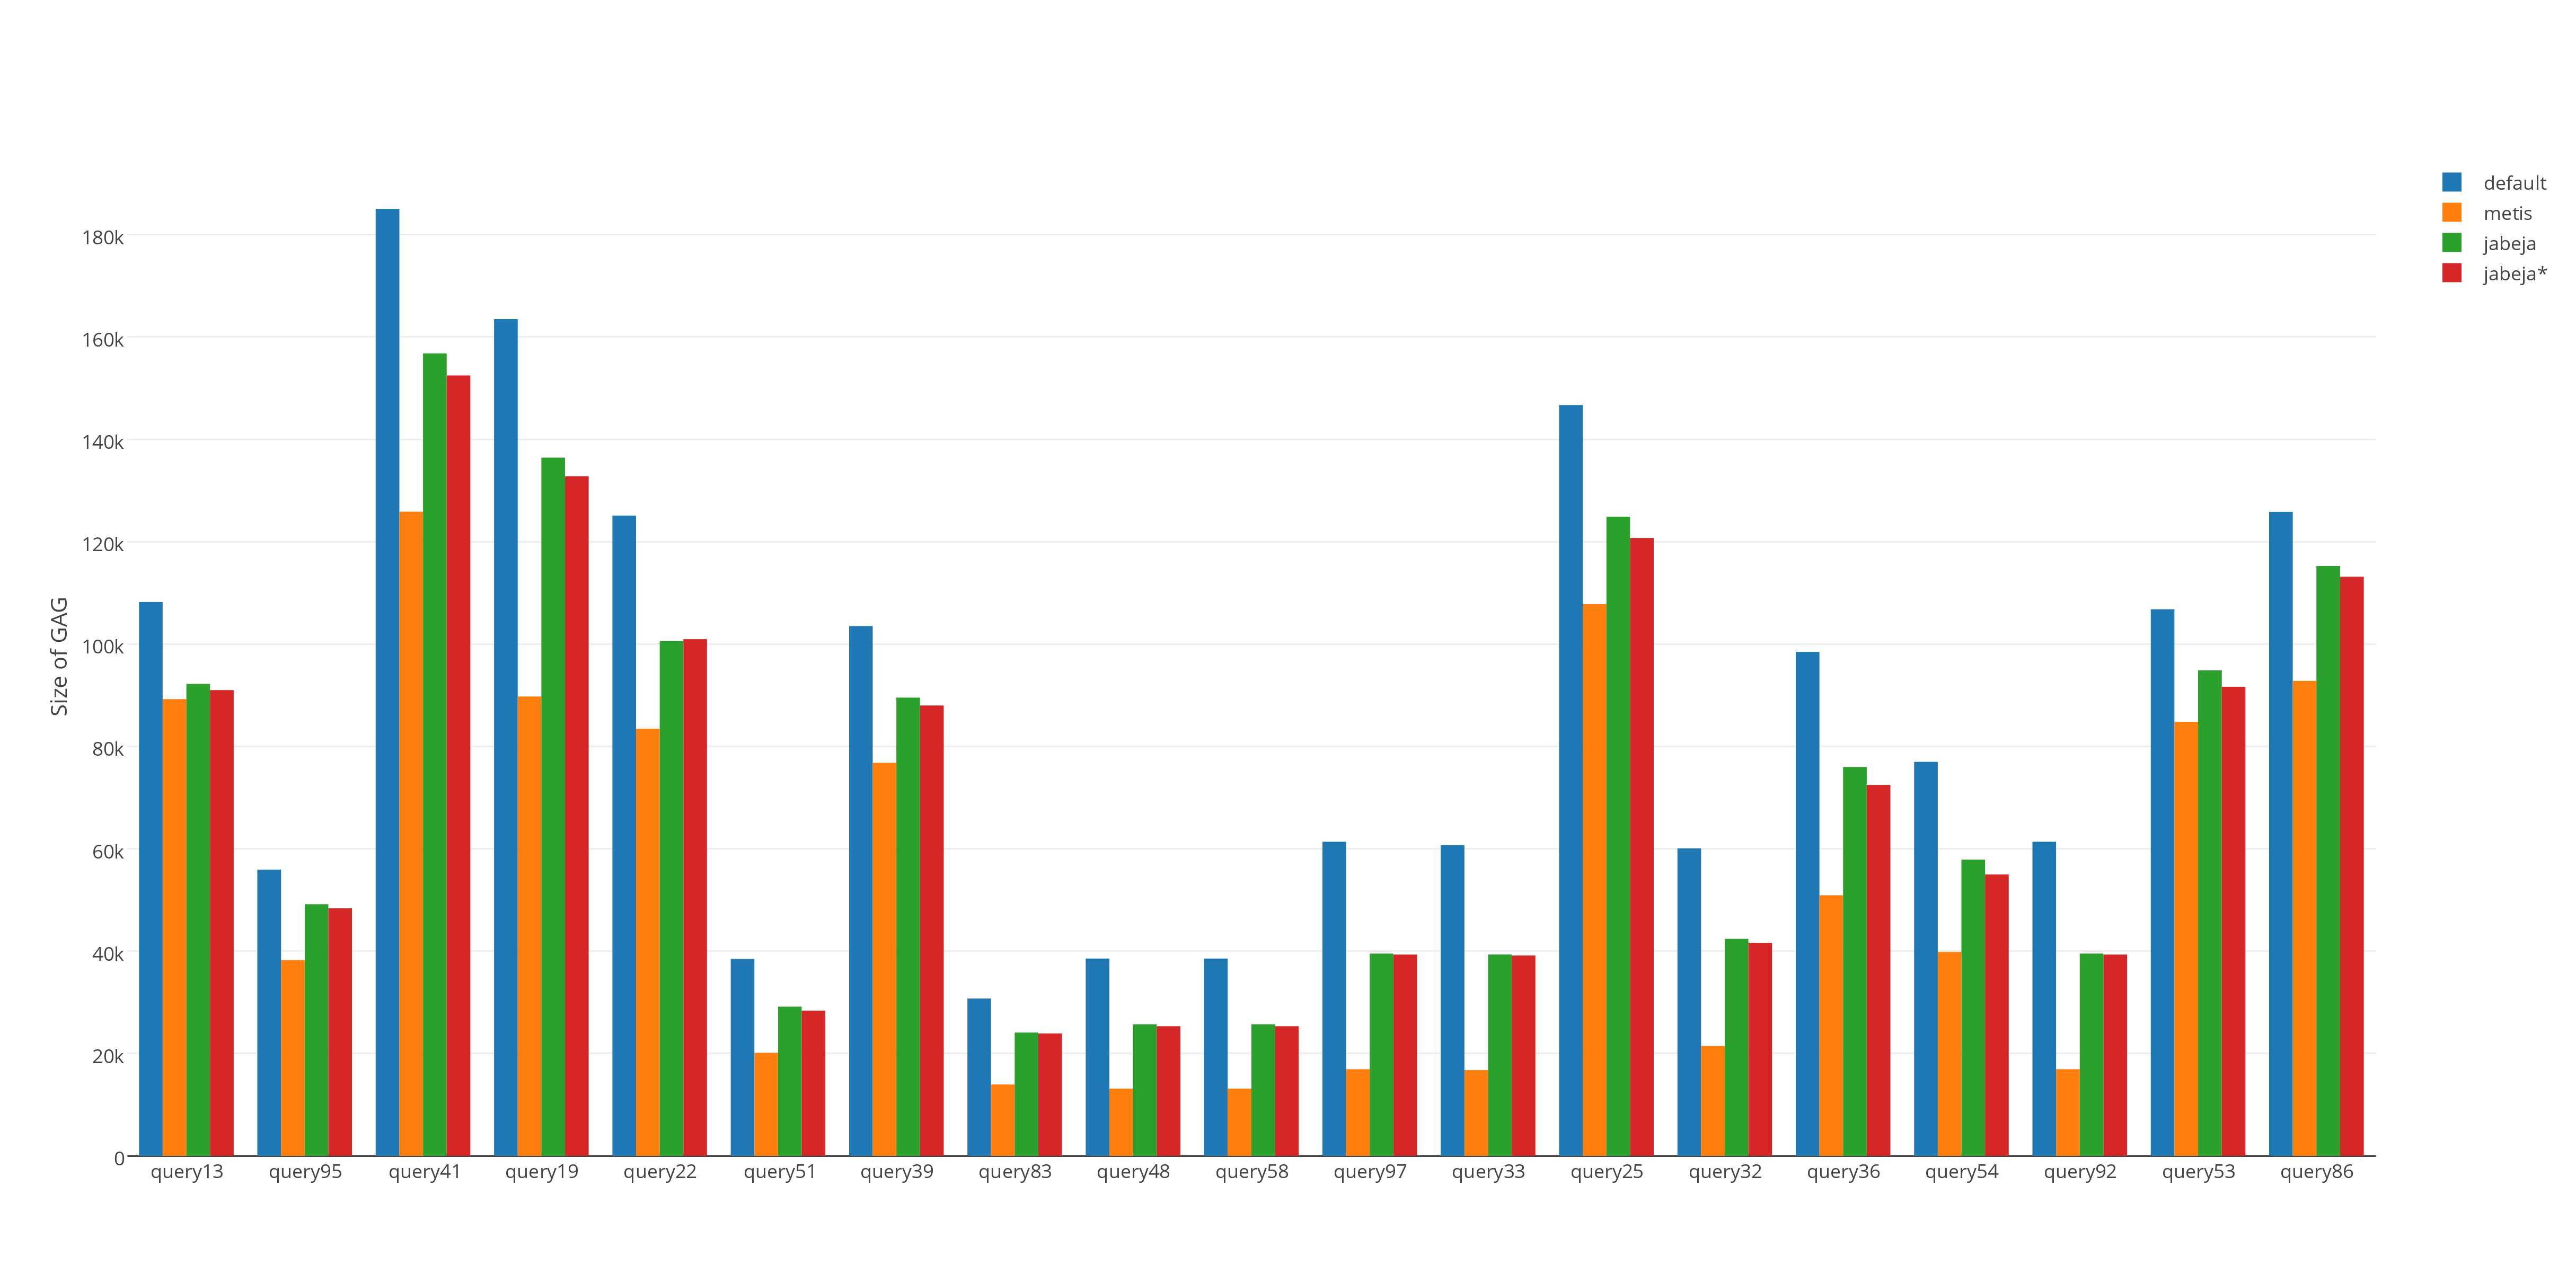
\includegraphics[width=1.0\textwidth]{img/gmark-01m-gag}
\end{figure}
\\The interesting findings are:
\begin{enumerate}
    \item The size of GAG is correlated with the number of input-nodes:
    \begin{enumerate}
        \item METIS has least input-nodes, which also leads to the small size of GAG.
        \item JABEJA* has fewer input-nodes and much more cross-edges than JabeJa, but it still produces the smaller size of GAG.
        \item Default partitioner is worst in GAG size, which is also consistent with the number of input-nodes.
    \end{enumerate} 
    \item The number of nodes in the GMark Graph doesn't influence the relevant results of different partition strategies since it's observed that all those three diagrams are in the same shape.
\end{enumerate}
\begin{figure}[h!]
  \caption{GAG size of GMark Graph ($10^6$ nodes)}
  \label{fig:gmark-1m-gag}
  \centering
    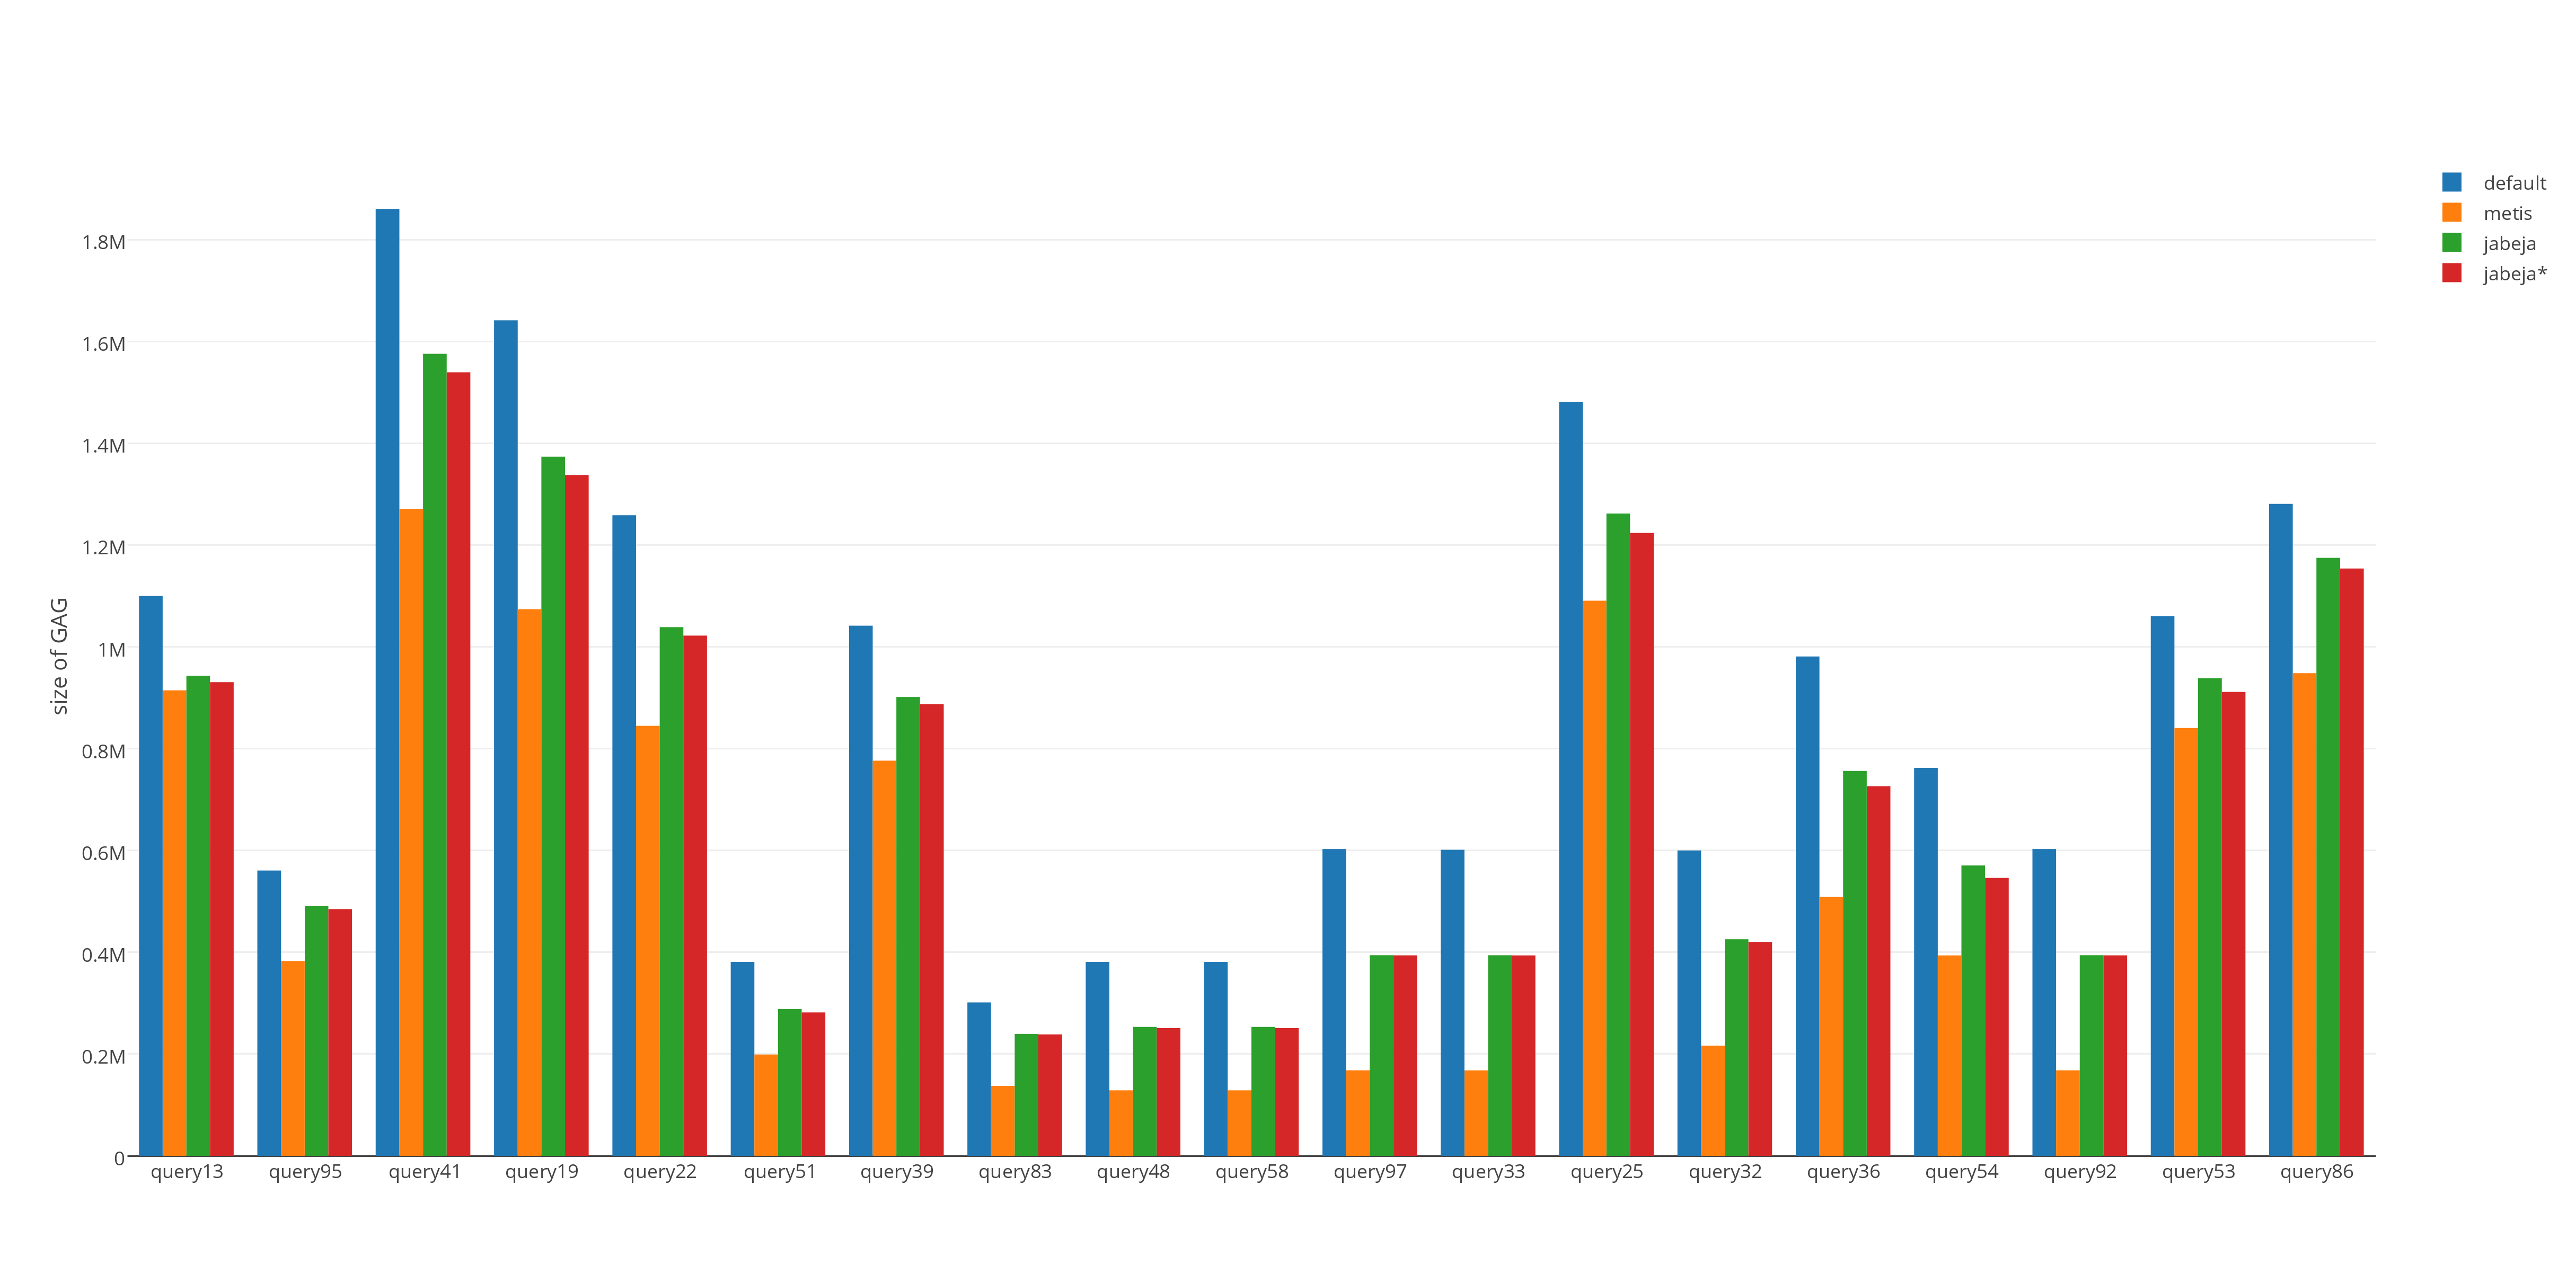
\includegraphics[width=1.0\textwidth]{img/gmark-1m-gag}
\end{figure}
\begin{figure}[h!]
  \caption{GAG size of GMark Graph ($10^7$ nodes)}
  \label{fig:gmark-10m-gag}
  \centering
    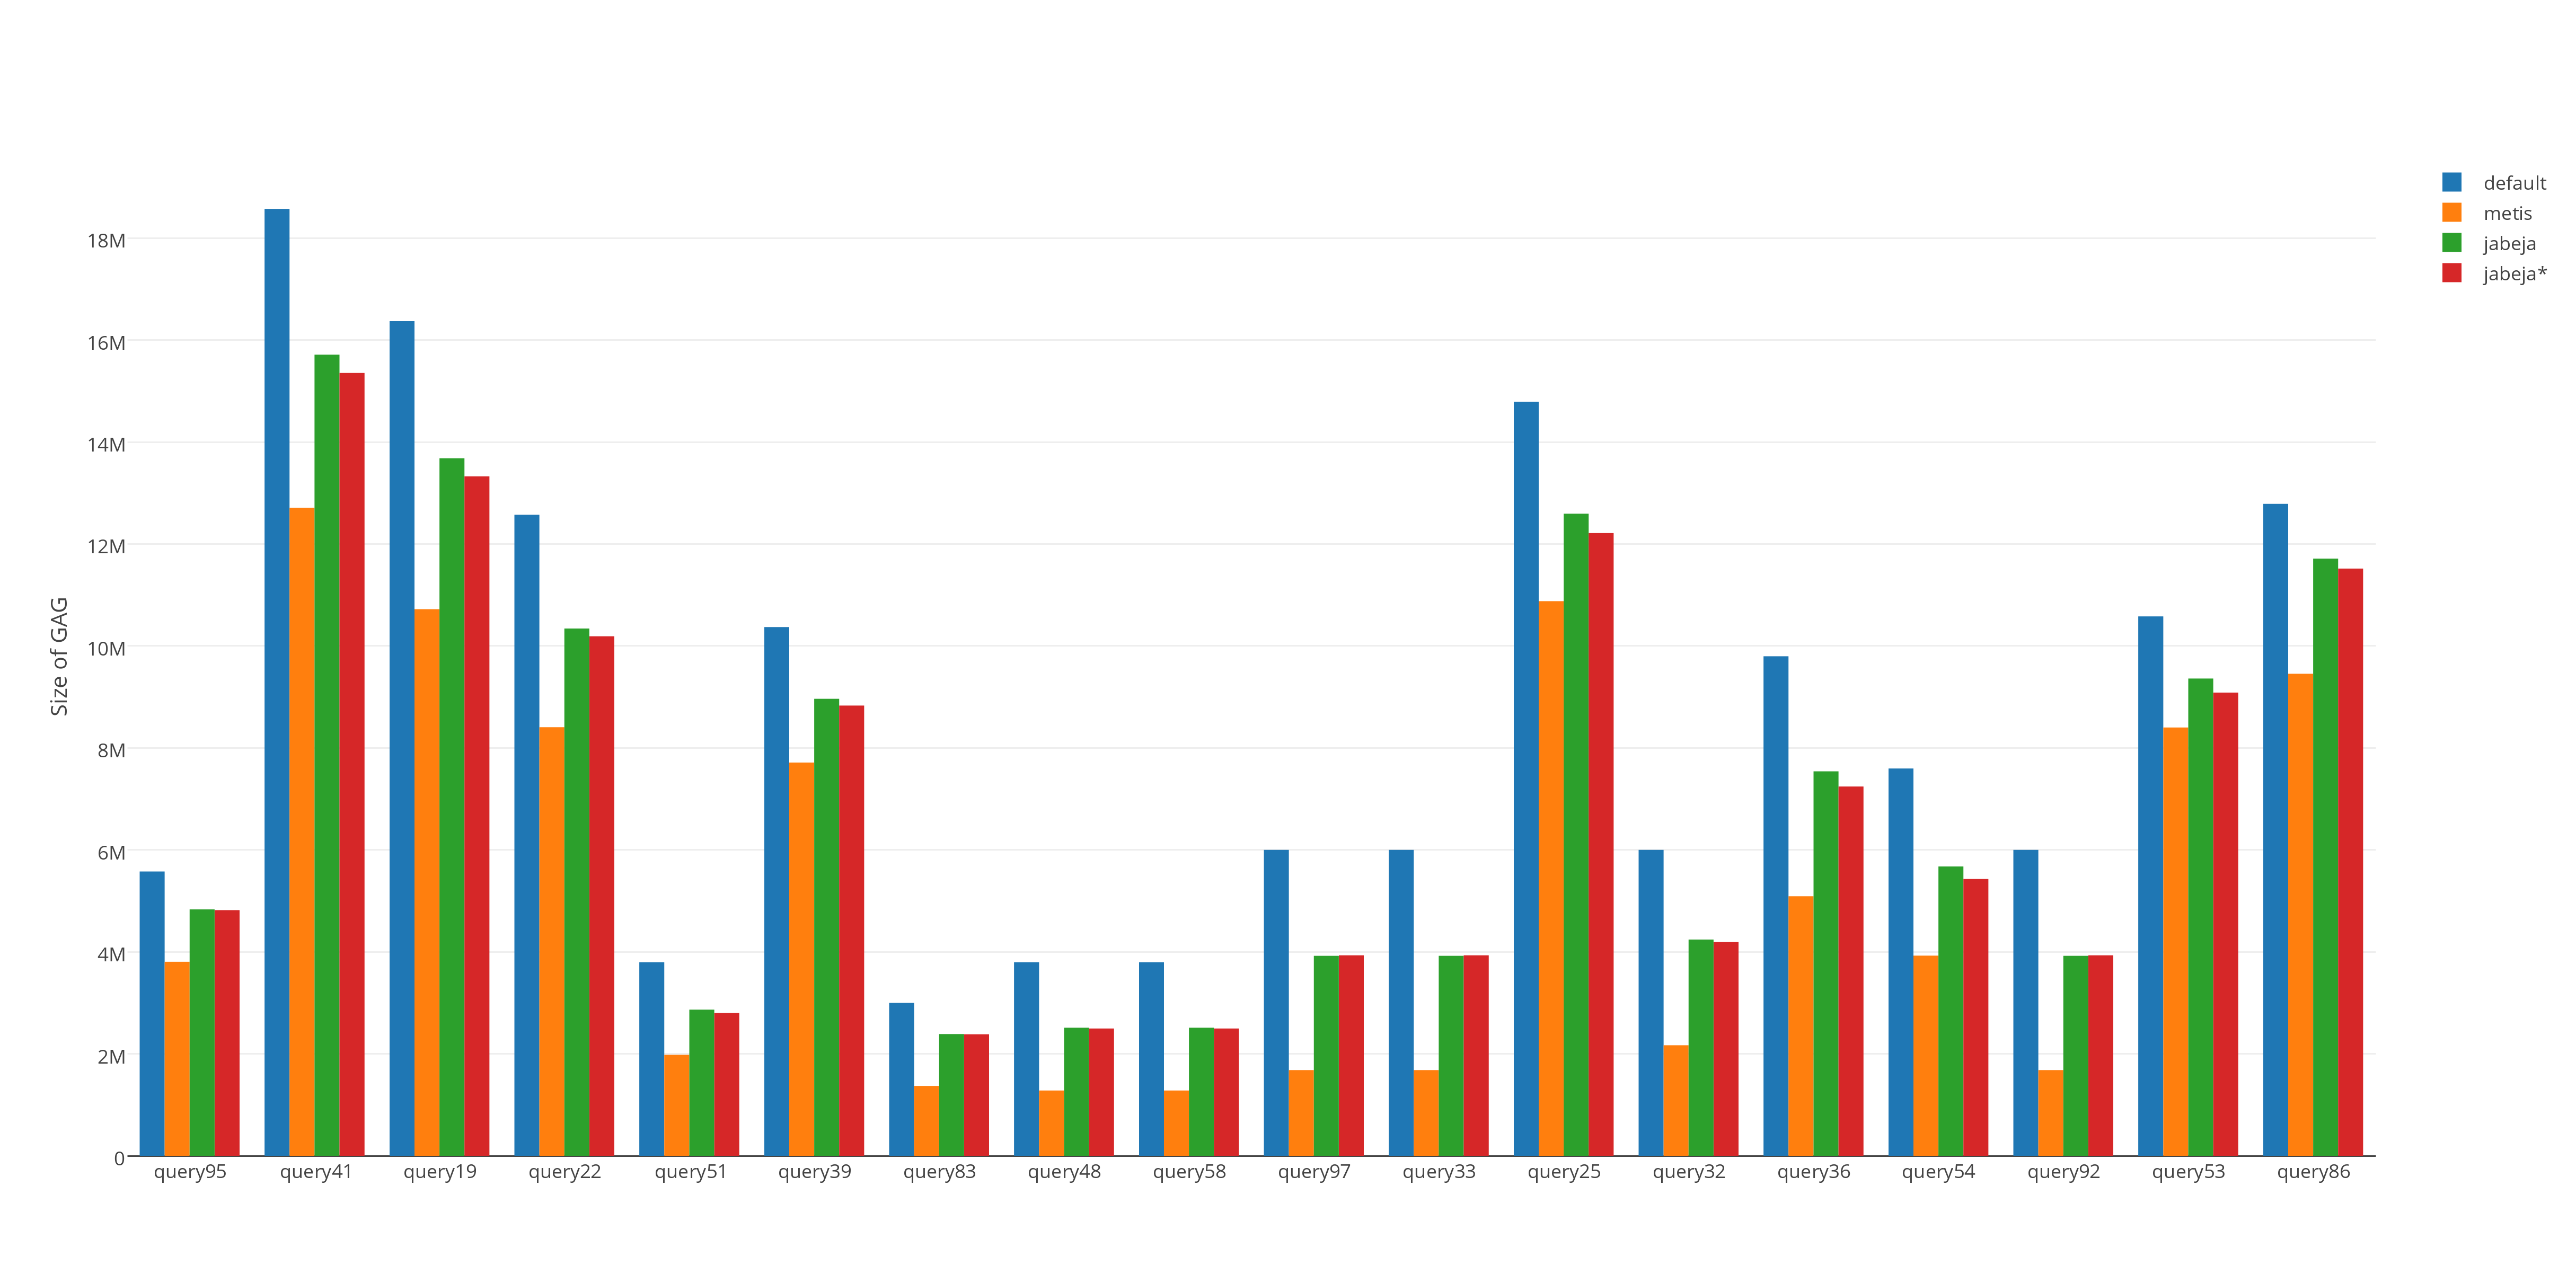
\includegraphics[width=1.0\textwidth]{img/gmark-10m-gag}
\end{figure}
We can see that in general METIS, JABEJA and JABEJA* are all improving the size of GAG to some extent. In the best case, the METIS could reduce the size of GAG to $30\%$, which could release the communication pressure during collecting GAG to driver significantly.

\subsection{Driver Computation Time}
Another reason of reducing the GAG size is that by pushing more work to executor side, the computation time on the driver side should be cut down accordingly. The time spent in the driver is described in Figure \ref{fig:gmark-01m-driver}, Figure \ref{fig:gmark-1m-driver} and Figure \ref{fig:gmark-10m-driver}. The x-axis is the index of queries in each benchmark and y-axis represents the time spent on the driver side in milliseconds.
\begin{figure}[h!]
  \caption{Driver Computation Time of GMark Graph ($10^5$ nodes)}
  \label{fig:gmark-01m-driver}
  \centering
    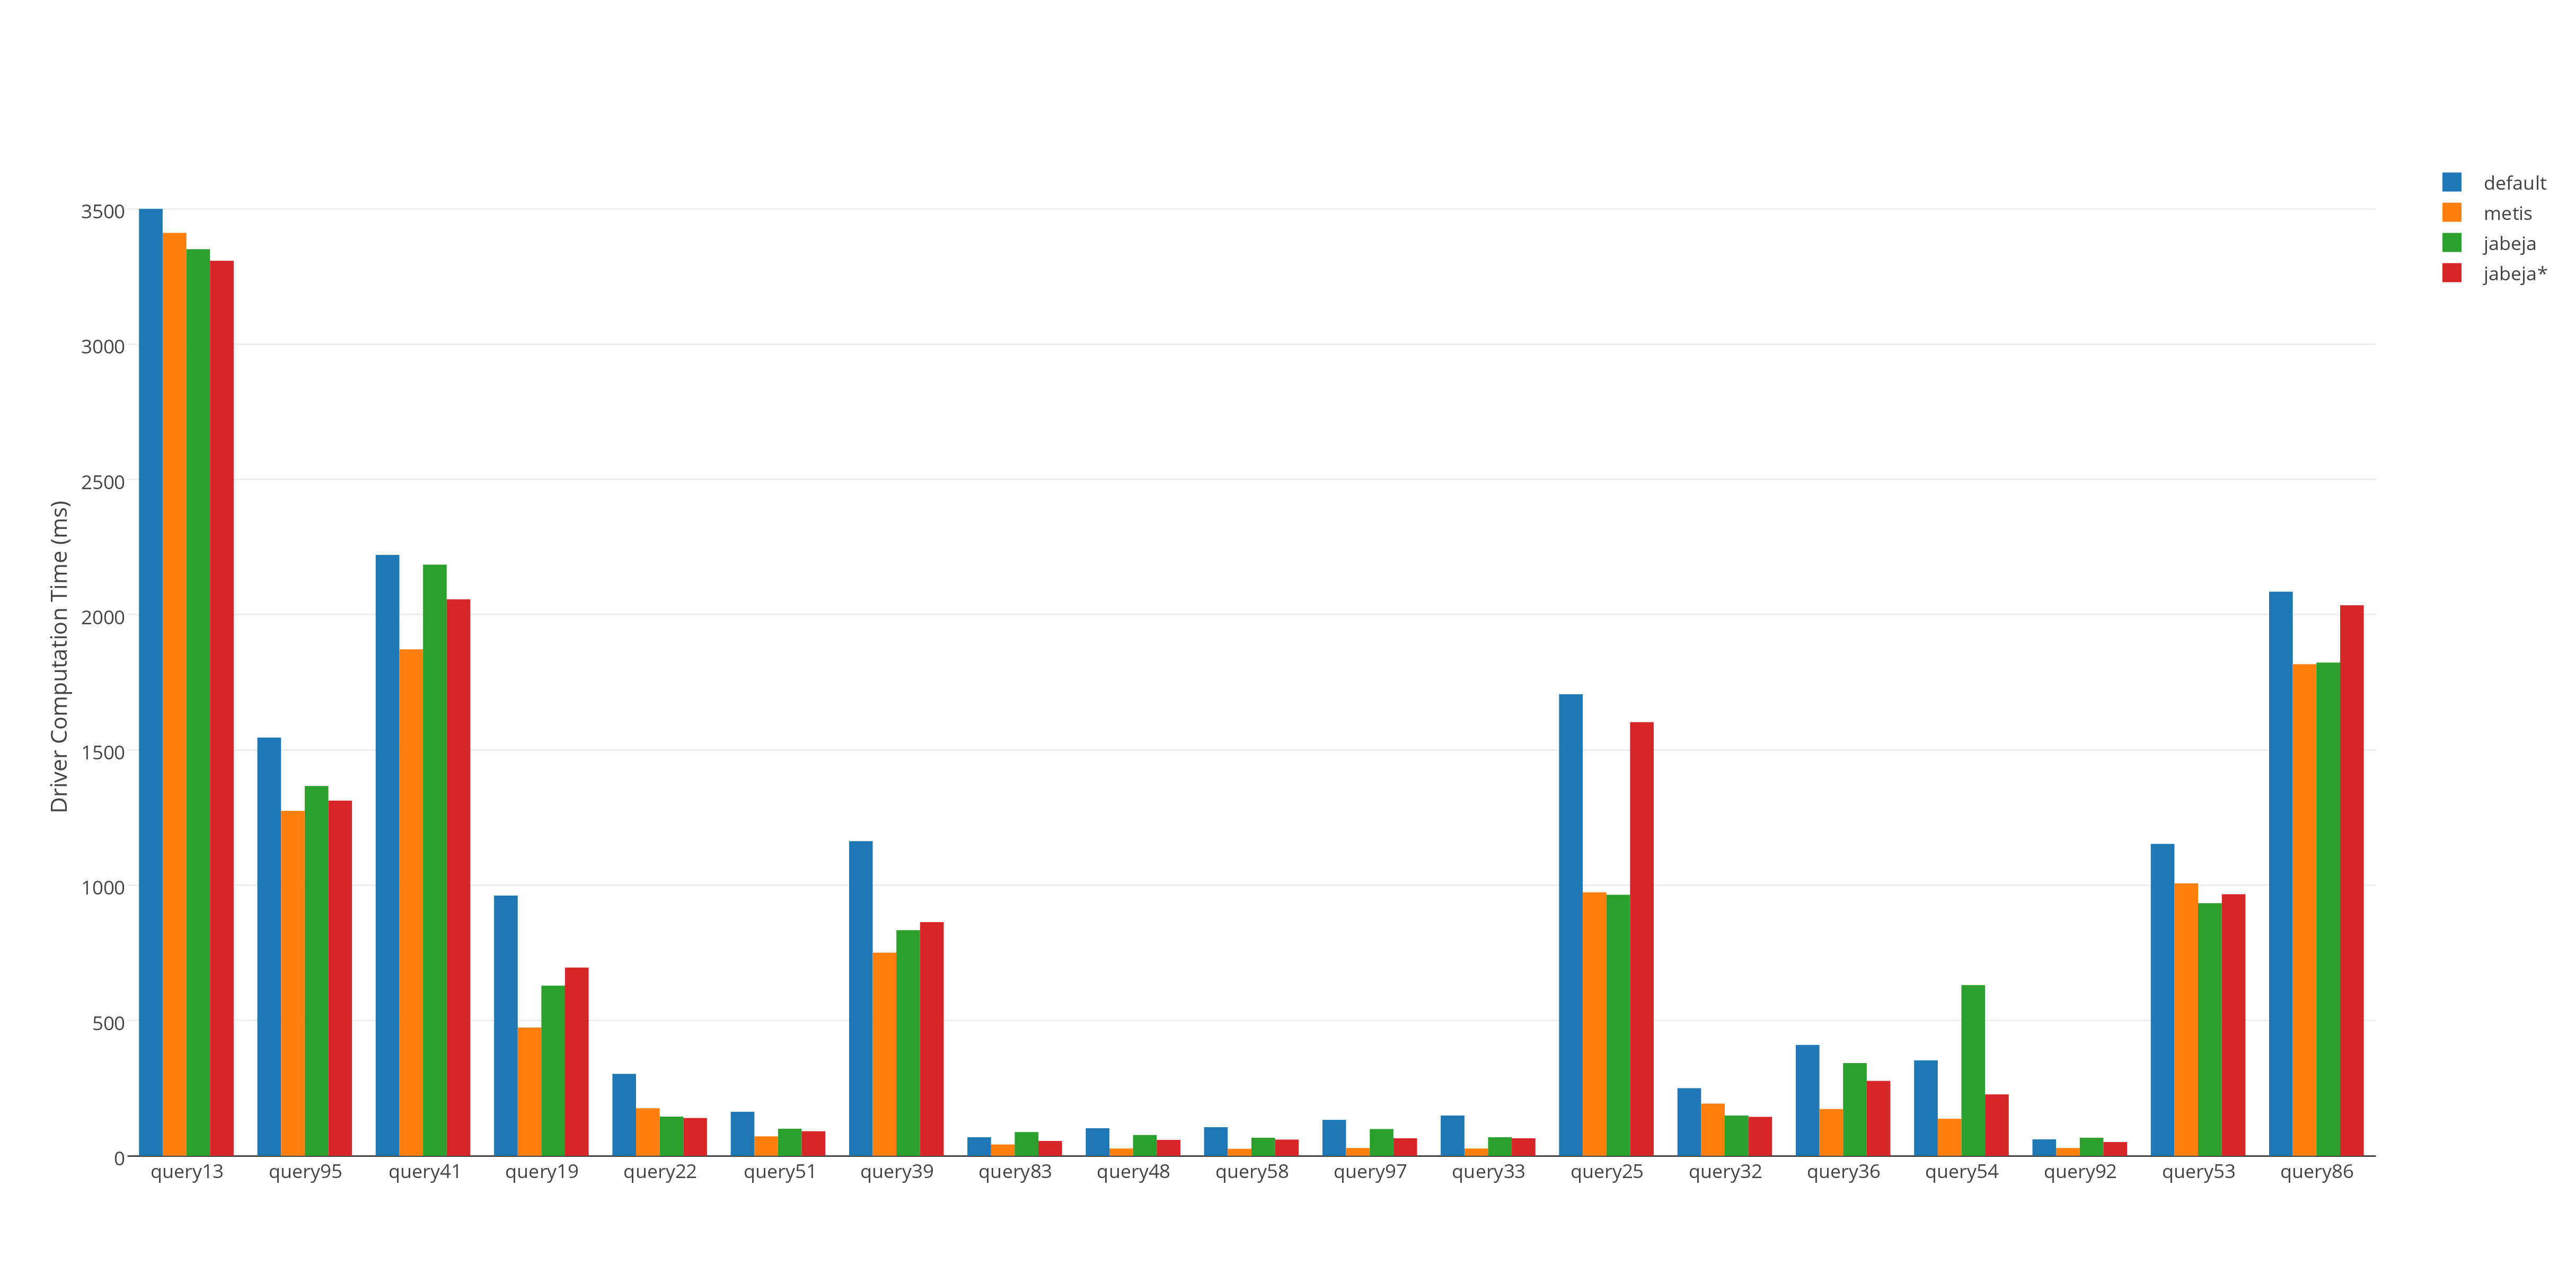
\includegraphics[width=1.0\textwidth]{img/gmark-01m-driver}
\end{figure}
\begin{figure}[h!]
  \caption{Driver Computation Time of GMark Graph ($10^6$ nodes)}
  \label{fig:gmark-1m-driver}
  \centering
    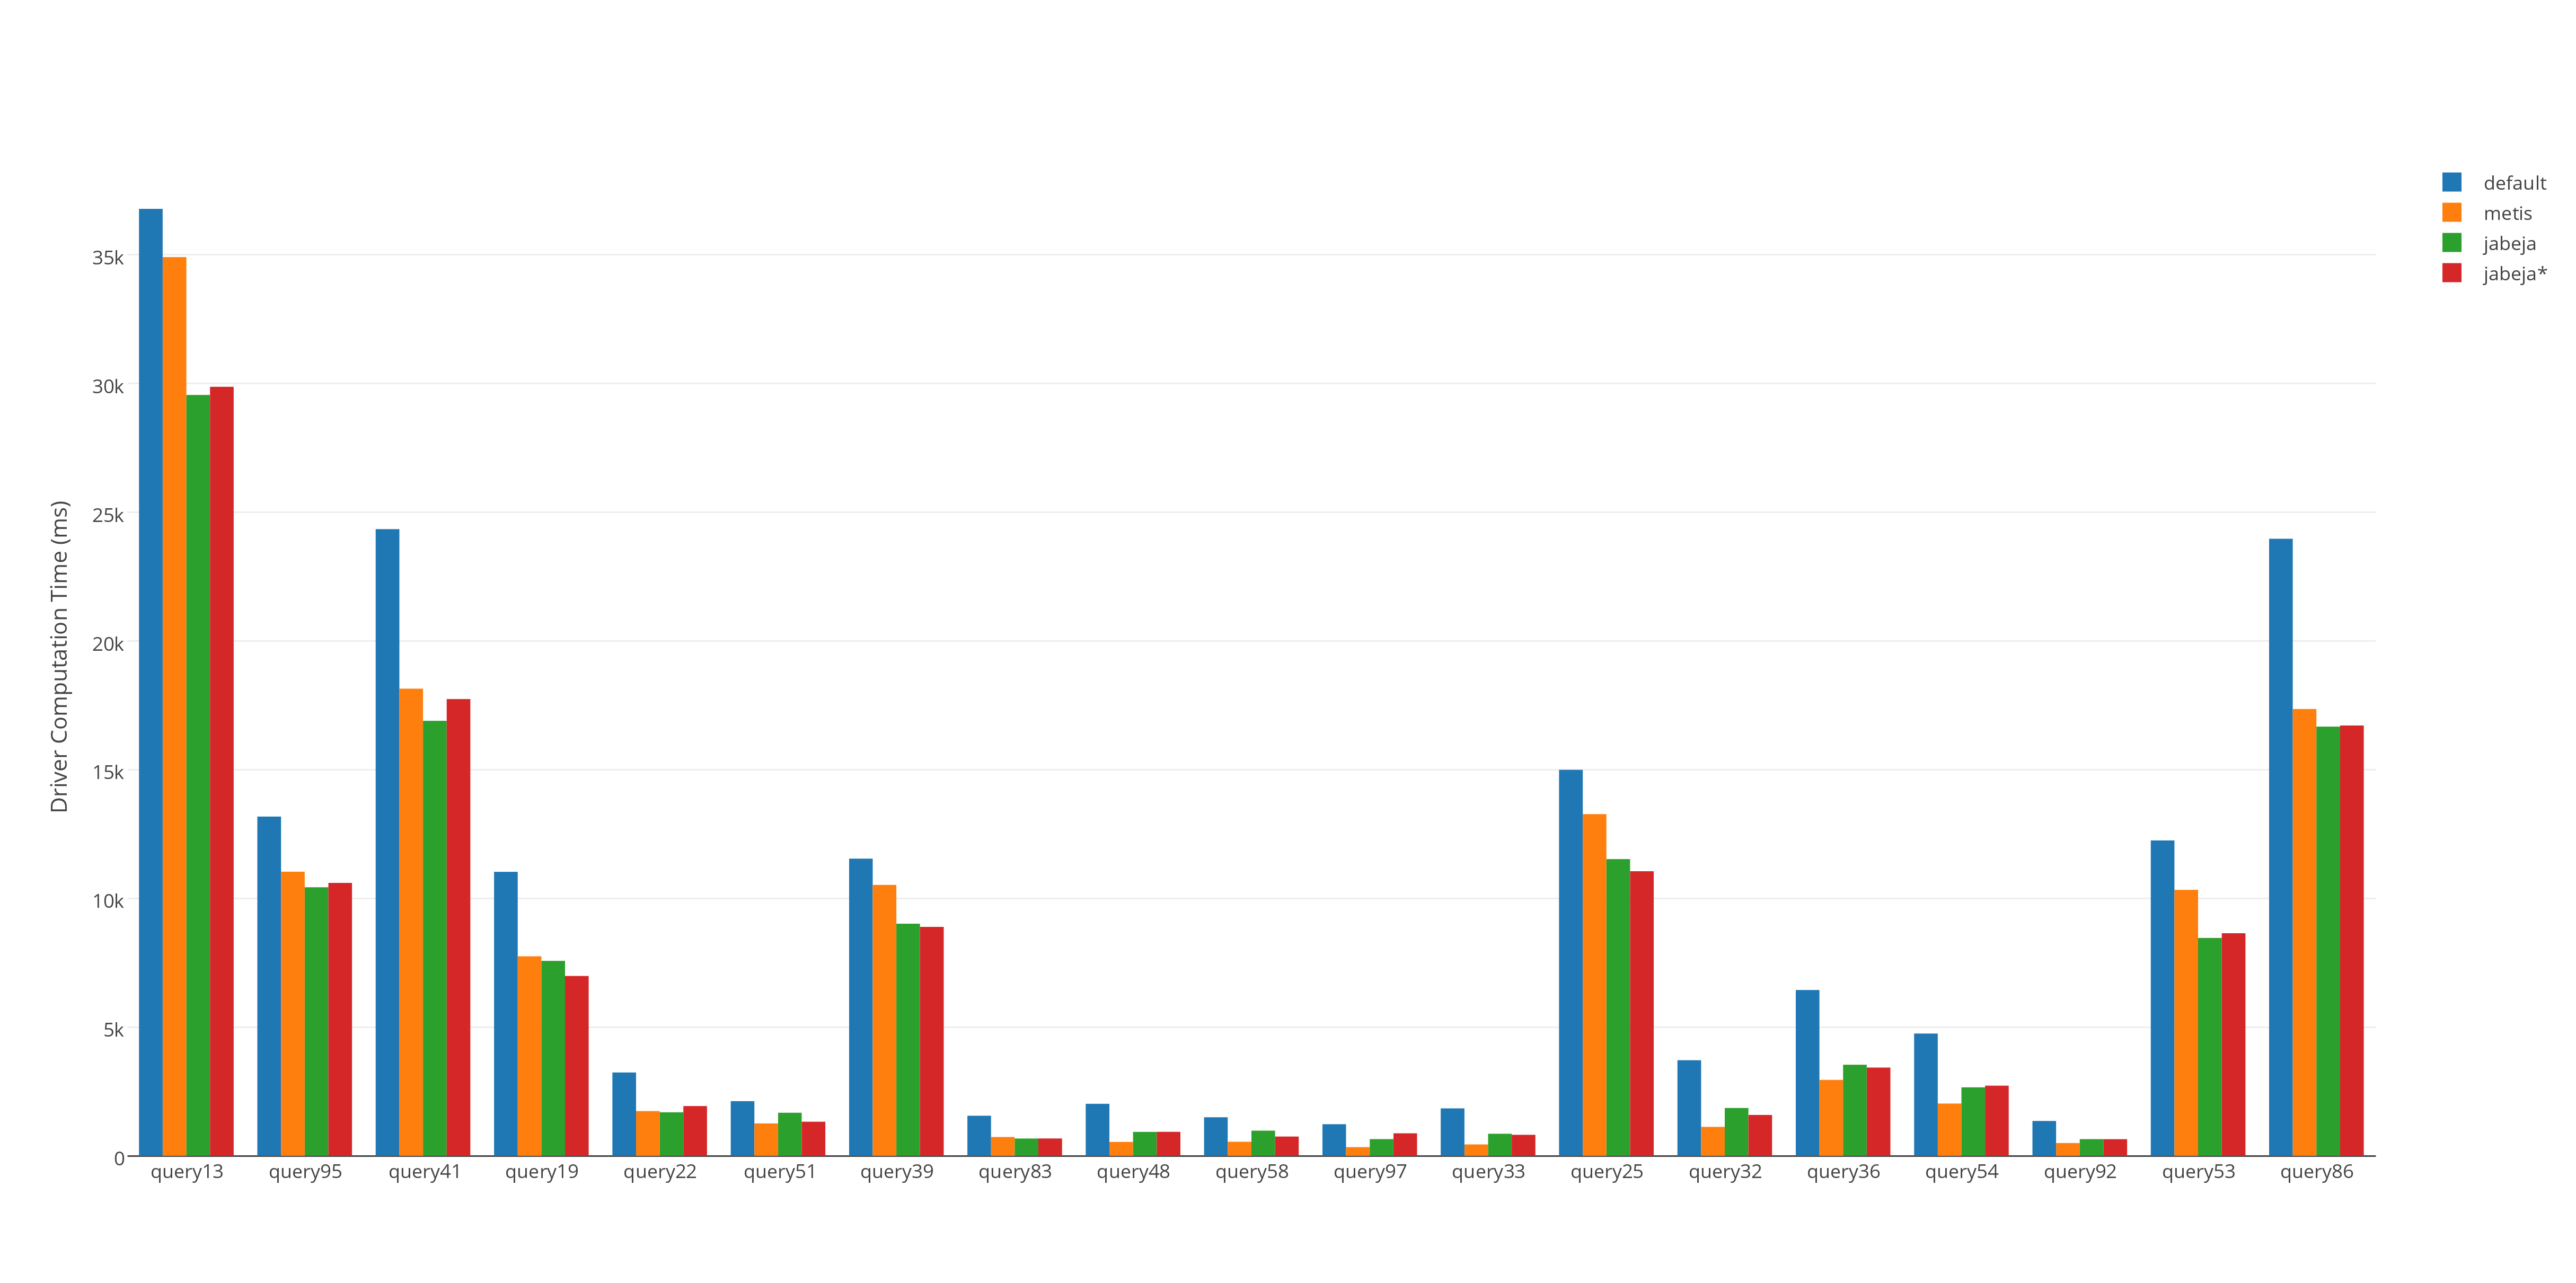
\includegraphics[width=1.0\textwidth]{img/gmark-1m-driver}
\end{figure}
\begin{figure}[h!]
  \caption{Driver Computation Time of GMark Graph ($10^7$ nodes)}
  \label{fig:gmark-10m-driver}
  \centering
    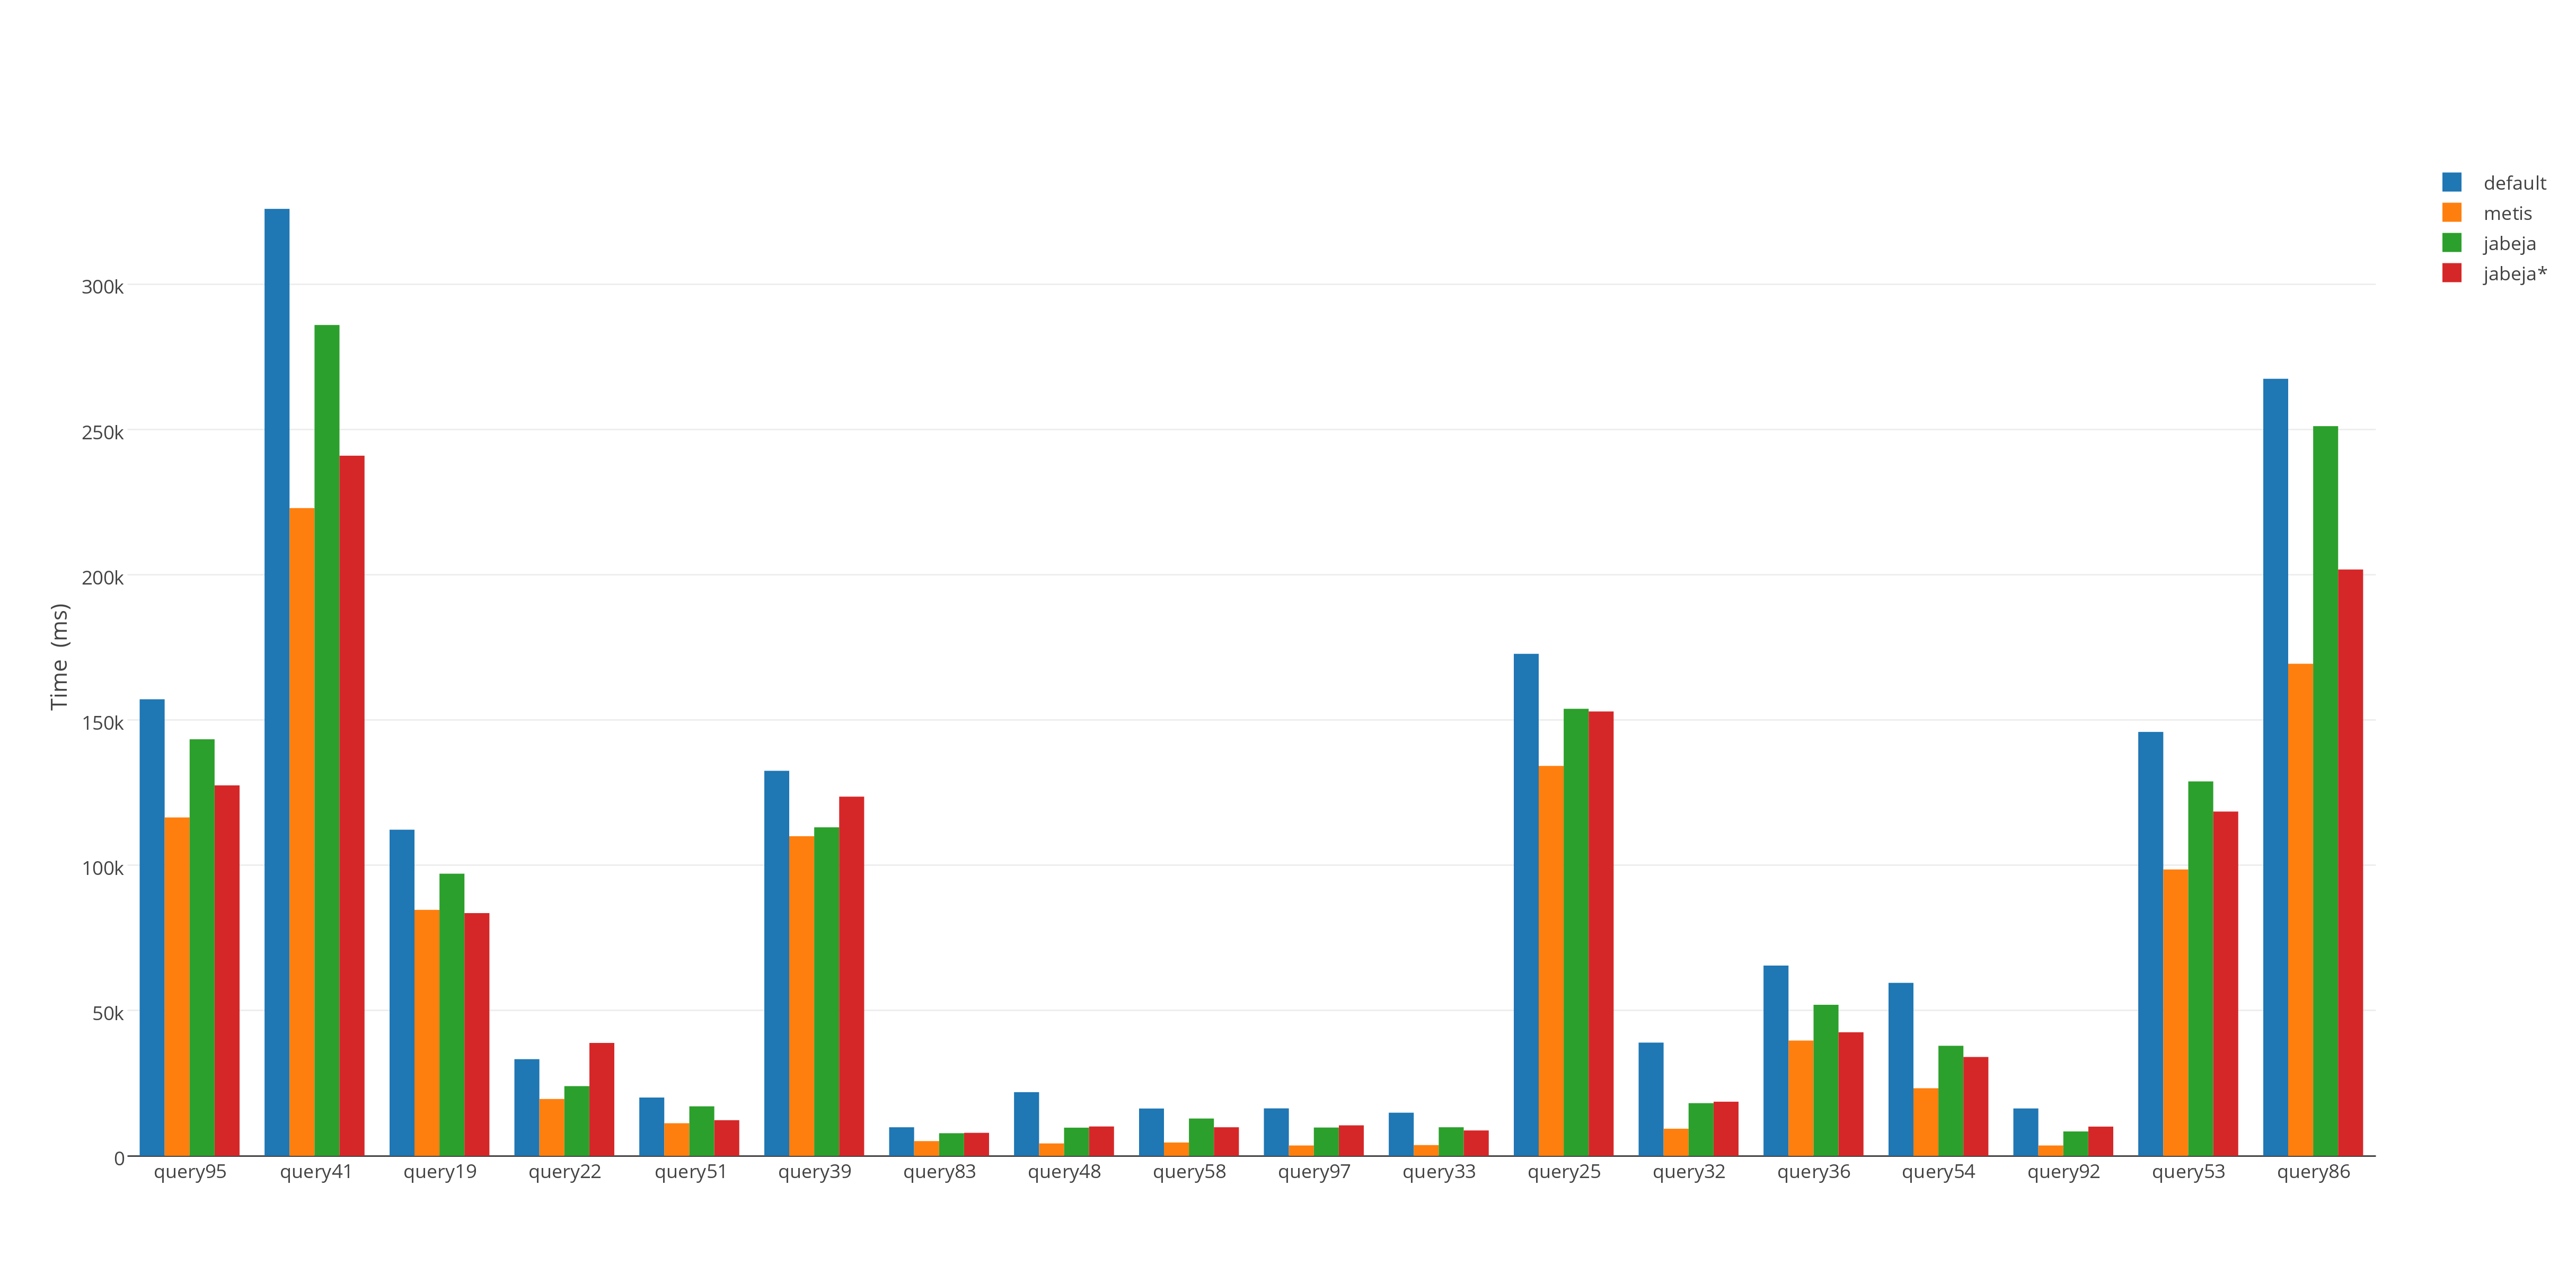
\includegraphics[width=1.0\textwidth]{img/gmark-10m-driver}
\end{figure}
The observations are:
\begin{enumerate}
    \item In most cases, the driver calculating time is consistent with the number of input-nodes and size of GAG.
    \item For some specific queries, such as query25 and query86 in Figure \ref{fig:gmark-01m-driver}, the JabeJa* takes more time than JabeJa. The reason behind is that although the size of GAG is similar, the computation time depends on the query itself and structure of GAG. Furthermore, the computation time only takes a few seconds, which means the reduced GAG size might not compensate the difference in the GAG structure. With increasing size of GAG, the special cases appear much less and when the nodes number is $10^7$, driver computation time of all queries are almost consistent with the trend of GAG size.
\end{enumerate}
\subsection{Overall Running Time}
Recall that in the Figure \ref{fig:alibaba-dan-jobs}, the driver computation can take more than $50\%$ percent of total time during evaluation. One of the goals of improving the partition strategies is to minimize the overall time. So besides the metrics we have already discussed above, we would like to investigate if the smart partition strategies are improving the total time spent on evaluation. The final result is list in Table \ref{overall-time}.
\begin{table}[h!]
\centering
\caption{Overall running time per query}
\label{overall-time}
\begin{tabular}{l|ll}
\hline
\#Nodes & strategy & time (ms)\\
\hline
\multirow{4}{*}{$10^5$}               & default & 95384  \\
                                      & METIS   & 74846  \\
                                      & JabeJa  & 86117  \\
                                      & JabeJa* & 76209  \\
\hline
\multirow{4}{*}{$10^6$}               & default & 43789  \\
                                      & METIS   & 63904  \\
                                      & JabeJa  & 58970  \\
                                      & JabeJa* & 69195  \\
\hline
\multirow{4}{*}{$10^7$}               & default & 505354 \\
                                      & METIS   & 562181 \\
                                      & JabeJa  & 289112 \\
                                      & JabeJa* & 404669 \\
\hline
\end{tabular}
\end{table}
According to the table, there are several key findings:
\begin{enumerate}
    \item The overall running time of size $10^5$ is consistent with the number of input-nodes or size of GAG. There are several queries which have driver-side bottleneck and are improved significantly.
    \item The overall running time of size $10^6$ is completely in contrast to the trend in the number of input-nodes. This is because we remove the queries with driver-side bottleneck as they take too much time to evaluate sequentially, and the rest of queries don't have such bottleneck (The time spent on the driver side is less than $10\%$ for all the queries). Then, compared  to the few seconds ahead on driver side, the overhead brought by more iterations in the distributed system is the dominant factor.
    \item The overall running time for size $10^7$ is in between the previous two situations: There are no queries which invest more than $90\%$ time on driver side, but the average proportion of time spent on driver still increases compared to the graph of $10^6$ nodes.
\end{enumerate}
In Table \ref{driver-queries}, we list several queries that have the driver-side bottleneck. It could be observed that the larger ratio driver time has, the bigger improvement in overall time could partition-strategies achieve.
\begin{table}[] \small
\centering
\caption{Durations for Queries having Driver-side Bottleneck in ms}
\label{driver-queries}
\begin{tabular}{l|ll|ll|ll|ll|}
        & \multicolumn{2}{c|}{default} & \multicolumn{2}{c|}{METIS} & \multicolumn{2}{c|}{JabeJa} & \multicolumn{2}{c|}{JabeJa*} \\ \cline{2-9} 
        & driver        & overall      & driver      & overall      & driver       & overall      & driver       & overall       \\ \hline
query79 & 1131742       & 1184438      & 583344      & 684098       & 723931       & 774945       & 743393       & 797520        \\
query95 & 157175        & 467259       & 116484      & 395386       & 143382       & 311311       & 127518       & 411474        \\
query41 & 325978        & 1203186      & 222985      & 901448       & 285998       & 682628       & 241008       & 678135        \\
query19 & 112272        & 890674       & 84667       & 706296       & 97117        & 414311       & 83557        & 554804       
\end{tabular}
\end{table}
\subsection{Answers for Research Questions}
\subsubsection{Research Question 1}
In most cases JabeJa* performs better than JabeJa but still worse than METIS. The reason behind this might be the choice of parameters: the algorithm finds 5 random nodes when there is no optimal neighbor to swap color.  The number might be still too small in the large graph, and put the program into a local optimum. In some quick tests, increasing this parameter to 30 can improve the quality significantly. However, as the implementation is sequential and only simulates the result, it takes too long to run with such random nodes.  Besides, we do not use any sampling policies such as in \cite{awan2006distributed} and \cite{dowling2012shuffling}. 
\subsubsection{Research Question 2}
The size of GAG decreases for different benchmarks, and for each benchmark in various sizes with the decreasing number of input-nodes. In all cases, reducing the number of input-nodes can formulate a better structure for graph and lessen the quantity of GAG states collected to the driver.
\subsubsection{Research Question 3}
In most cases, the declining size of GAG can result in less time spent on the driver, but when the GAG sizes are close, the computation time may depend on the structure of GAG and query itself.
\subsubsection{Research Question 4}
The speedup in overall time depends on the proportion of time spent on the driver. For those queries with driver-side bottleneck, reducing GAG size can lead to significant decrease in overall running time.
\section{Summary}
In this chapter, we firstly look into the reasons for the bottleneck on driver side when running Dan Suciu's Algorithm. Based on the idea that smart partition strategies can optimize the performance, we looked into the relationships between different metrics such as the number of input-nodes, the size of GAG and running time. The existing partition strategies and one modified strategy are clustered and tested against multiple benchmarks. Based on final results of the experiments, smart partition-strategies can optimize the size of GAG, the data collected in the network and the driver performance significantly by reducing the input-node size.